\documentclass[12pt,a4paper,openright,twoside]{book}
\usepackage[utf8]{inputenc}

\newcommand{\thesislang}{english}
\usepackage{thesis-style}

% version
\newcommand{\versionmajor}{0}
\newcommand{\versionminor}{1}
\newcommand{\versionpatch}{2}
\newcommand{\version}{\versionmajor.\versionminor.\versionpatch}

\begin{document}
	
\frontmatter

% ! TeX root = thesis-main.tex
\title{Title}
\author{Francesca Neri}
\date{\today}

\newgeometry{margin=0.8in}
\begin{titlepage}
	\begin{center}
		% \vspace*{0.2cm}
		
		\large
		\textbf{ALMA MATER STUDIORUM -- UNIVERSITÀ DI BOLOGNA \\ CESENA CAMPUS}
		\\
		\noindent\hrulefill
		\vspace{0.4cm}
		
		%\Large
		Department of Computer Science and Engineering - DISI \\
            \vspace{0.1cm}
        %\Large
		Second Cycle Degree in Digital Transformation Management \\
            \vspace{0.1cm}
            Class: LM-91
		
		\Large
		\vspace{4cm}
		\textbf{
			% The Role of Enterprise Performance Management \\ 
   %          in Modern Businesses: A Case Study of Oracle \\
   %          Cloud EPM Implementation
            Leveraging Oracle Cloud EPM Business Rules \\
            for Efficient Planning: Insights and \\
            Implementation Strategy
		}
		
		\large
		\vspace{2cm}
		Graduation thesis in \\
		\vspace{0.2cm}
		\textsc{BIG DATA AND CLOUD PLATFORMS}
		
		\vspace{5.5cm}
		\begin{minipage}[t]{0.64\textwidth}
			\begin{flushleft}
				Supervisor \\
				\vspace{0.2cm}
				\textbf{Prof. Matteo Francia}
			\end{flushleft}
		\end{minipage}
		\begin{minipage}[t]{0.34\textwidth}
			\begin{flushright}
				Candidate \\
				\vspace{0.2cm}
				\textbf{Francesca Neri}
			\end{flushright}
		\end{minipage}\\
		
		\vfill
		\noindent\hrulefill
		\vspace{0.3cm}
		\large
		
		I Graduation Session
		\\
		Academic Year: 2022-2023
	\end{center}
\end{titlepage}
\restoregeometry


\begin{acknowledgements}

This thesis is linked to my curricular internship for the final examination carried out at PricewaterhouseCoopers (PwC) from January to March 2023.
%
During the internship experience at PwC Italy, I worked in the advisory-transformation Line of Service, cooperating with the Enterprise Performance Management - Financial Service (EPM-FS) team.

The EPM-FS team works for the main players in the financial sector and deal with business transformation projects which are aimed at re-engineering and optimizing the company's internal processes.

Along the internship period, I worked directly with the EPM team in a project concerning the Oracle Cloud EPM platform.
%
This project is addressed to an Italian Corporate Group which has more than 7,000 points of sale around the world. 

Due to corporate policy, the name, data and information of the Corporate Group to which the project is addressed, cannot be disclosed. 
%
It is important to note that respecting the privacy and confidentiality of companies' data is critical in maintaining their trust and credibility.
%
Therefore, throughout this thesis, I will be referring to the company only in general terms and avoiding the use of any identifying information or data. \\

I would like to express my gratitude to PwC Italy for this opportunity, to the entire EPM team for welcoming me and making me feel like a part of the team, and my supervisor for his guidance and support throughout the internship. \\

To be continued...

\end{acknowledgements}

\begin{abstract}	

This thesis explores the role of Enterprise Performance Management (EPM) solutions in modern businesses, ranging from planning, reporting and forecasting purposes. 
%
The project was carried out using Oracle Cloud EPM, a cloud-based platform developed by Oracle Corporation, that offers an integrated suite of financial and operational planning and analysis tools.

The thesis starts by providing an overview of Enterprise Performance Management and its importance in modern businesses. 
%
It then delves into the benefits of using a cloud platform for EPM, including lower costs, increased flexibility, and easier scalability.

The main focus of the thesis regards the exploration of how financial and operational processes are integrated in a single EPM solution, whilst using data coming from different sources. 
%
The project involved working with a real-world client to identify the company planning needs and
then manipulating dimensions, elements, and hierarchies to meet those needs.
%
The techniques used to create customized planning models for the client will be analyzed, including the use of pre-built templates and the creation of custom calculations and formulas.

In addition to the technical aspects of the project, this thesis also explores the business benefits of using an integrated EPM solution, including better decision-making, improved financial performance, and increased visibility into operational processes.

Overall, the goal of this project is to provide a detailed exploration of the role of EPM solutions in modern businesses, with a focus on the importance of using a cloud platform and integrating financial and operational processes in a single solution. 
%
The project, carried out using Oracle Cloud EPM, provides a practical example of how businesses can leverage EPM solutions to improve their financial and operational planning and analysis capabilities.

\end{abstract}

\begin{dedication}
Optional. Max a few lines.
\end{dedication}

% \begin{acknowledgements}
% Optional. Max 1 page.
% \end{acknowledgements}

%----------------------------------------------------------------------------------------
\tableofcontents   
%\listoffigures     % (optional) comment if empty
%\lstlistoflistings % (optional) comment if empty
%----------------------------------------------------------------------------------------

\mainmatter

%----------------------------------------------------------------------------------------
\chapter{\introductionname}
\label{chap:introduction}
%----------------------------------------------------------------------------------------

In today's highly competitive business environment, effective performance management is essential for organizations to achieve their strategic goals and stay ahead of the competition.
%
With the advent of digital transformation, companies are now offered with huge opportunities from which they can benefit.
%
It is an inevitable change that organization must embrace to stay competitive and meet customer demands in the digital era.

One of the way to go in order to thrive among rivals in turbulent markets is to excel at various performance dimensions. 
%
One of the prerequisites for this is to be able to effectively manage and measure corporate performance using various performance management and measurement systems. 
%
These systems help companies to continuously react and adapt to external changes.

Enterprise and corporate performance and management methods can be viewed as the seamless integration of managerial systems. 
%
Each method should be embedded with business analytic operations like correlation, segmentation, regression and predictive analysis.
%
Performance management provides valuable data and insights that can help businesses make informed decisions by identifying trends, anticipating issues, and making adjustments to their strategy as needed.

Enterprise Performance Management (EPM) is an integral part of the success of modern enterprises as it helps organizations to gain visibility into their performance and to identify areas of improvement.
%
It is a management approach that integrates multiple business processes and systems to enable organizations to plan, measure, analyze, and optimize their performance.

 Enterprise Performance Management enables businesses to improve strategic decision-making, maximize their productivity and achieve the desired business results while ensuring that expenses are minimized and that the best use of resources is made.
 %
 It assists businesses to effectively forecast and plan for their future financial performance, helping them to ensure compliance and reduce risk. 
 
 The advantages of EPM are numerous and make it a valuable tool for organizations of all sizes.

 The aim of this thesis is to investigate the role of EPM in modern businesses and the benefits and challenges of implementing EPM solutions. 
 %
 Specifically, this thesis will focus on a case study of Oracle Cloud implementation in a business to illustrate how EPM solutions can improve organizational performance. 
 
 Oracle Cloud is a leading cloud-based EPM solution that provides organizations with a comprehensive suite of financial and operational performance management applications.
 %
Oracle Cloud EPM provides a flexible and scalable solution that can meet the needs of organizations of all sizes.
%
It offers various tools and solutions that allow companies to plan, budget, forecast, and report on their financial and operational performance.
%
The implementation of an Oracle Cloud EPM solution involves a series of steps throughout which organizations must work closely with their implementation partner to ensure that the solution is tailored to their specific needs and requirements.

Using a cloud platform to implement an EPM solution can provide numerous benefits for the organization. 
%
One of the primary advantages regards the ability to access critical data and applications from anywhere and at anytime.
%
Additionally, cloud platforms can help reduce costs associated with maintaining on-premises infrastructure and provide scalability and flexibility to meet changing business needs. 
%
Cloud-based EPM solutions also enable organizations to leverage the latest technologies and innovations without having to worry about managing and upgrading hardware and software. 
%
Cloud providers typically offer high levels of security and compliance, which can help organizations protect sensitive data and maintain regulatory compliance. 

%
\paragraph{Thesis Structure.}
%

Accordingly, the reminder of this thesis is structures as follows:
%
\Cref{chap:introduction} will provide an overview of the background and significance of the topic, scope and limitations of the study, and an overview of the methodology.
%
\Cref{chap:background} will review the literature on Enterprise Performance Management, including the definition and concepts of EPM and its evolution in modern businesses. 
%
It also provides an overview on Oracle Cloud and its EPM solutions, together with the benefits and challenges of implementing EPM in businesses. 
%
\Cref{chap:design} will describe the approach and methodology used for the implementation of and EPM solution to a company.
%
\Cref{chap:implementation} will present the case study of Oracle Cloud implementation in a business, including the company background and context, EPM solution selection and implementation process, key features and functionalities of the implemented EPM solution, impact of the EPM solution on the company's performance, and the best practices for EPM implementation. 
%
Finally, \Cref{chap:conclusions} concludes the thesis summarizing the main concepts ans discussing the implication for theory and practice.

\section{Background and significance of the study}

Enterprise Performance Management is a management approach that involves using data and analytics to monitor, measure, and improve an organization's performance. 
%
It integrates various management processes, including financial planning, budgeting, forecasting, risk management, and performance measurement, to help organizations align their goals with their strategies and improve their overall performance.
%
To access and analyze data more quickly and accurately, organizations typically use software applications that automate and streamline this process.

These application often include dashboards, pre-built report templates and other tools that provide real-time insights into organizational performance.

The ultimate goal of EPM is to help organizations to achieve their strategic objectives and optimize their performance, whether that be in terms of financial performance, customer satisfaction, operational efficiency, or other key performance indicators. 
%
By using data-driven insights and decision-making, EPM enables organizations to more effectively manage risks, allocate resources, and make strategic decisions that improve their overall performance and competitiveness in the marketplace.

Enterprise Performance Management operates within a complex and dynamic business environment, characterized by a number of key trends and challenges. 
%
One of the most significant trends in recent years has been the growing adoption of cloud technology for enterprise applications, including EPM. 

Cloud-based EPM solutions offer many advantages over traditional on-premises systems, including greater scalability, flexibility, and accessibility, as well as lower costs and reduced IT complexity. 
%
As a result, more and more organizations are turning to cloud-based EPM solutions to improve their performance management processes.

Another key trend in modern business is the growing importance of data-driven decision making. 
%
With the increasing availability of data and advanced analytical tools, organizations are able to gain deeper insights into their operations and performance, and make more informed decisions. 
%
EPM plays a critical role in this trend by providing real-time insights into organizational performance and enabling managers to make data-driven decisions that align with their strategic goals. 
%
This helps organizations to be more proactive in identifying and responding to performance issues, and to optimize their operations and resources to achieve their desired outcomes.

In addition to these trends, EPM also operates within a business environment that is constantly evolving and adapting to changing market conditions. 
%
The need for businesses to be agile and responsive to these changes is an ongoing challenge, and EPM can help address this by providing a flexible and adaptable framework for performance management. 
%
By monitoring key performance indicators and providing real-time insights into performance, EPM enables businesses to quickly identify and respond to changes in market conditions, and to make strategic decisions that keep them ahead of the competition.

Overall, the context in which EPM operates is characterized by a rapidly evolving business environment, where technology, data, and agility are critical to success. 
%
Enterprise Performance Management plays a critical role in helping organizations to adapt to these trends and challenges, by providing a data-driven and agile approach to performance management that enables them to optimize their operations, resources, and strategic decision making.

\section{Scope and limitations of the study}

The scope of the project includes different areas of focus that range from the definition of Enterprise Performance Management, its benefits, its implementation in companies and the future trends.
%
The thesis starts by defining what Enterprise Performance Management is and how it differs from the other management approaches in place.

Then, the project investigates the potential benefits that EPM can bring to modern businesses including enhanced decision-making, better alignment of business objectives with strategies, increased efficiency and improved performance.
%
It then explores the challenges associated with implementing EPM solutions in businesses which, for example, include issues related to data collection and analysis, performance measurement, reporting and the use of technologies and specific software.
%
Data is the core element of a performance management system; in order to have accurate reports and effective forecasts, it is important to have large quantities of data which which the EPM system is populated. 

The project aims at analyzing a case study regarding the implementation of an EPM solution in a company.
%
Then, it explores the future trends and challenges that are likely to impact the role of Enterprise Performance Management in relation with emerging technologies, changing business models, and evolving business needs and expectations.

There are some limitations related to the study that should be taken into account.
%
Such limitations include both extrinsic and intrinsic elements of the project, ranging from the access to large amounts of data, the complexity of the topic investigated and the diversity of applications involved.

More in details, in order to explore the impact of Enterprise Performance Management on businesses, it may be necessary to have access to data related to business performance belonging to different organizations.
%
However, in this thesis we will analyze a case of implementation carried out for a specific company which operates in a specific industry sector. 
%
Of course, each company has its own characteristics in terms of operations and business management, which impact the implementation of the solution and its overall effectiveness.
%
Also, modern businesses vary widely in terms of size, sector, business model and many other factors.
%
In particular, the activities of management and performance control carried out by the company have a significant impact on how the EPM solution will be implemented and maintained.
%
Of course, there is no single solution that can be applied to any business but they vary according to the needs of the company.
%
As a result, it can be difficult to generalize findings in one type of business to other types of businesses.

\section{Overview of the methodology}

The methodology applied to the implementation of an Enterprise Project Management solution follows some key steps and best practices that depend on the specific requirements of the client company, the size and complexity of the project and the available resources.
%
The entire implementation process is built together with the client company which is responsible for assessing the quality of each step and ensuring the compliance with the requested features of the system.

The project begins with a planning phase, during which the company's business needs and goals are identified and the scope of the project is defined.
%
This involves identifying the objectives and key deliverables of the project, as well as any constraints or assumptions that will impact the implementation.
%
During this phases, it is important to identify the stakeholders by determining who will be impacted by the implementation and what their needs and requirements are.
%
Another key element in the planning phase is the definition of success criteria in order to measure the outcome by using performance indicators.
%
Finally, a clear and detailed project plan is developed, outlining the timeline, the budget, and resources required to complete the implementation.

Then, during the solution design phase, the EPM solution is designed based on the identified business requirements and goals, including the configuration of the environment, customizing features and workflows, and integrating with other systems.

The development and testing phase is the core part of the project.
%
In this phase the EPM solution is built and configured, relying on a process of continuous feedback from the customer.
%
Both individual components and the solution as a whole are tested to ensure that they meet the business requirements and goals.

After that, the client company's personnel which will use the system is trained through training sessions, user manuals, and other resources to help users understand the system and use it effectively.

Finally, the solution is deployed to the client's company environment.
%
If applicable, the data of the old system will be migrated into the new one, which will be integrating with additional existing systems.
%
After the EPM solution is deployed, configured and permissions are set, ongoing support and maintenance are provided to ensure the system runs smoothly and meets the company's needs.
%
This involves providing technical support, troubleshooting issues, and applying updates to keep up with the software advancements.

%----------------------------------------------------------------------------------------
\chapter{Literature Review}
\label{chap:background}
%----------------------------------------------------------------------------------------

\section{Definition and concepts of Enterprise Performance Management}

\section{The evolution of EPM in modern businesses}

\section{Oracle Cloud and its EPM solutions - TO DROP}

 % Oracle Cloud EPM customers have experienced 61% improved forecast accuracy and are more likely to connect their financial plans with supply chain, sales, project, and workforce planning (Oracle, Value of EPM Survey, 2022). 

 %https://blogs.oracle.com/modernfinance/post/leader-gartner-magic-quadrant-financial-planning-software-epm

\section{Benefits and challenges of implementing EPM in businesses}

%----------------------------------------------------------------------------------------
\chapter{Methodology}
\label{chap:design}
%----------------------------------------------------------------------------------------

The successful implementation of an Enterprise Performance Management (EPM) system can have a significant impact on the performance and competitiveness of modern businesses. 
%
However, the implementation of such a system requires careful planning, preparation, and execution to ensure success. 

In this chapter, we will examine the methodology used in the implementation of a Oracle Cloud EPM solution for a company.
%
We will discuss the key steps involved in the implementation process, the needs and requirements of the company, what they want to achieve and how they plan to achieve it.

We will also explore specific approaches, methodologies, and tools used in each phase of the project, and discuss the challenges and lessons learned throughout the implementation. 
%
By examining the methodology used in this project, we can gain insights into best practices for Oracle Cloud EPM implementation and its unique features and tools.

\section{Scope and objectives of the project}

This project has been implemented for a global leader in high-end design with pro-forma revenues of \$ 960 million in 2022.
%
The company is characterised by an unparalleled portfolio of iconic Brands and a multi-channel distribution approach across the globe.
%
The Group’s mission is to provide long-lasting value for clients through an innovative manufacturing process carried out by the Brands which compose the Group.
%
It is composed of ten brands which own a total amount of ten factory locations in Italy, Spain, Denmark and US.
%
The Group has a presence in more than 130 countries with more than 7,000 points of sale worldwide. 
%
They created an exclusive network of highly professional dealers and mono-brand stores, consolidating its international presence with the opening of wholly owned flag-ship stores in leading capital cities around the world.

Their goal is to foster an ecosystem which enables their companies to grow into a strong worldwide presence with both reach and scale by curating a powerful and iconic culture across the Brands.
%
This ecosystem has been geared towards the success of each individual Brand, so that the Group invests its resources at Brand level, boosting the creative process and the customer experience.

By bringing together multiple Brands and helping them achieving their best, the Group is a global leader in an otherwise traditionally highly fragmented market of high-end design. 
%
With a strong cultural heritage, characterised by multi-channel distribution and diversified product categories, the Group has created a unique design hub, offering a platform with which carefully selected Brands can be accelerated to grow at scale through a well-defined strategic approach.
%
Their strategic pillars are:

\begin{enumerate}
    \item Brand desirability, making Brands more attractive, better known and sought after.
    \item Direct to consumers, enhance and personalize the customers’ experience, getting closer to end customers and the design community.
    \item International expansion, expand the geographical reach, boosting their presence in markets with high growth potential and building a strong position into mature ones.
    \item Contract business, strengthen the leadership in high-end Contract business, providing considerable added value to the overall quality of a project in the eyes of architects, designers, and developers.
\end{enumerate}

The management control department\footnote{Management control in a business refers to the processes and activities undertaken by a dedicated department to plan, monitor, and control organizational activities. The aim of management control is to align the actions of individuals and departments with the company's strategic goals and objectives, enabling effective decision-making, performance evaluation, and the optimization of resources.} of the holding Group is responsible for assessing the financial situation and evaluating the overall performance of the entities.
%
Their tasks and activities range from monitoring financial performance, tracking key performance indicators (KPIs), and identifying areas for improvement.
%
Prior to the implementation of the Enterprise Performance Management solution, the management control department faced significant challenges in accessing and consolidating financial data from across the Group's entities.
%
This made it difficult to accurately evaluate performance and to make informed decisions.
%
With the EPM solution, the management control department plans to improve data accuracy, streamline reporting processes, and gain real-time visibility into financial data across all entities. 
%
The final goal is to drive better decision-making and improve overall financial performance for the Group.
%
With better data, streamlined processes, and more accurate reporting, the management control department can make informed decisions that lead to growth and profitability for the Group. 
%
Additionally, the increased efficiency and productivity that comes with a cloud EPM solution can help to reduce costs and improve compliance and risk management.

The goal of the project is to implement a planning environment in Oracle Cloud EPM in which the data belonging to the different Brands of the Group are all integrated in a single view.

Therefore, the implementation project involves the deployment of a software solution that will enable the company to effectively manage its financial data, analyze it, and make informed business decisions.
%
In particular, the planning environment is used an maintained by the client's management control department so, along the implementation process, we interacted directly with the people working in that area.

The Corporate Group was born in 2018 and is the result of the aggregation of different companies which belong to the same industry sector.
%
The entities which compose the Group have a different story, a different culture, different business models and, as a consequence, different Group Control Models.

\begin{figure}[htbp]
	\centering
	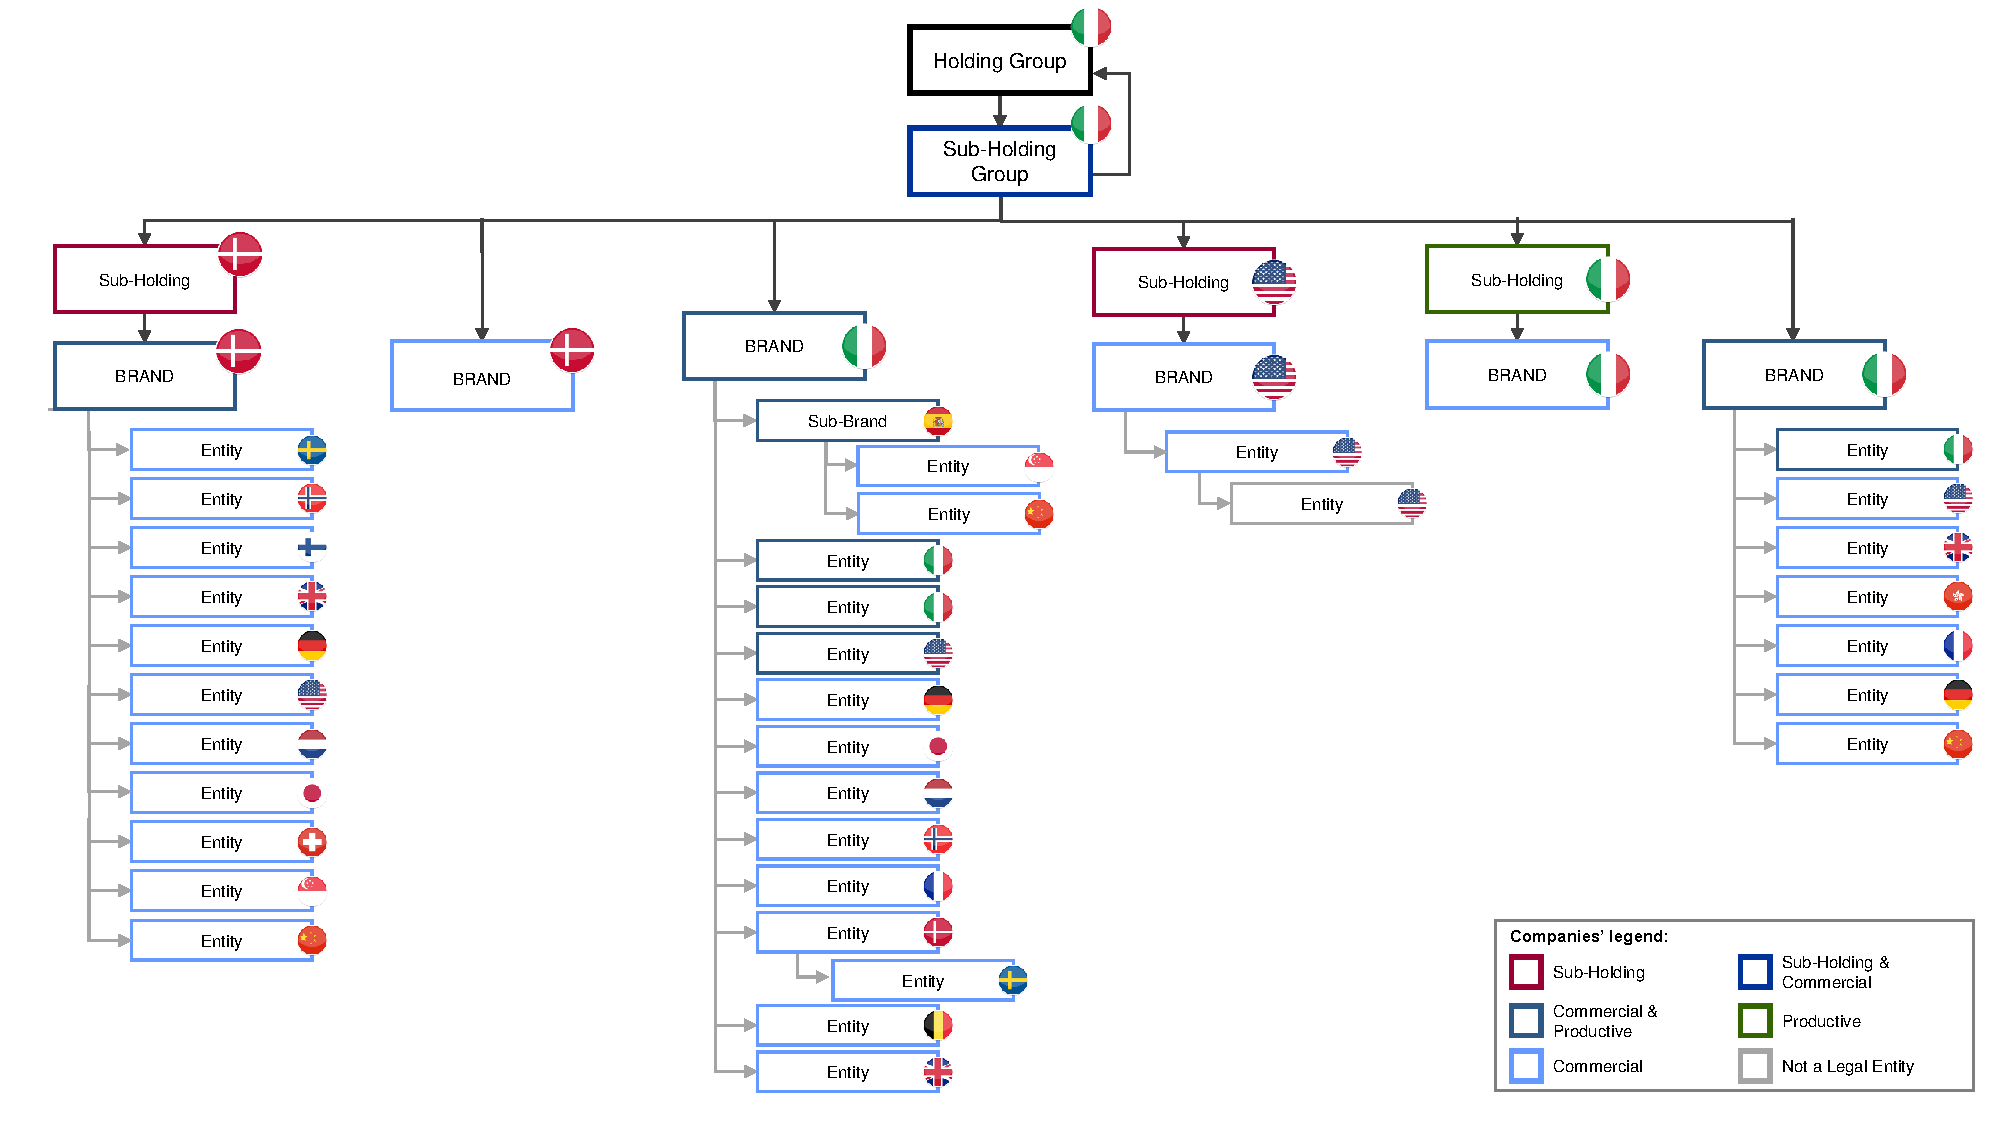
\includegraphics[width=\linewidth]{figures/structure.pdf}
	\caption{Structure of the Holding Group}
	\label{fig:structure}
\end{figure}

Since its creation, the new Group has planned several initiatives to facilitate the integration between the different realities.
%
The lack of organizational structure due to the different Group Control Models was considered as a key issue in sustaining the new planning and reporting needs of the Group.
%
To solve this issue, the Group started an activity of  homogenization of Enterprise Performance Management model of the entities, by:

\begin{enumerate}
    \item Defining a consolidated financial reporting;
    \item Defining a performance reporting system based on KPI’s;
    \item Defining a treasury reporting and rolling cash flow forecast process.
\end{enumerate}

\begin{figure}[htbp]
	\centering
	\includegraphics[]{figures/cycle.pdf}
	\caption{Enterprise Performance Management Framework}
    \floatfoot{Source: PricewaterhouseCoopers HK}
	\label{fig:cycle}
\end{figure}

Figure \ref{fig:cycle} represents the three main stages of Enterprise Performance Management, each pf which plays a critical role in managing and improving the performance of a business. 
%
The strategy phase is the foundation of the EPM cycle, where the business establishes its objectives and formulates its strategic plans. 
%
This phase involves the following key activities: objective setting, planning and budgeting.
%
Firstly, the business defines its short-term and long-term objectives, which could include revenue targets, market share goals, cost reduction objectives or customer satisfaction metrics.
%
Then, based on the objectives, the business develops a comprehensive plan to achieve its goals by identifying key initiatives, allocating resources, and setting timelines.
%
Finally, the business drafts a budget with the aim of allocating financial resources to different departments, projects or activities, ensuring that the financial plans align with the strategic objectives.
%
The outcome of the strategy phase is a well-defined roadmap that guides the organization's actions in the subsequent stages of the EPM cycle.

Then, the execution phase focuses on implementing the plans and strategies developed in the strategy phase and involves activities related to reporting, control, and performance tracking.
%
The business collects and analyzes data from various sources, such as financial and operational systems and then transform the data collected into meaningful reports and dashboards that provide insights into the organization's performance.
%
At the same time, through an attentive control process, the business makes sure that the defined plans and objectives are followed by monitoring key metrics, comparing actual results against targets, and taking corrective actions when necessary.
%
The execution phase is crucial for ensuring that day-to-day activities are aligned with the overall goals of the business.

Finally, the performance phase involves evaluating the organization's performance, calculating key performance indicators (KPIs), and deriving insights to drive continuous improvement. 
%
This is done by assessing the business performance against the objectives set in the strategy phase and by calculating KPIs to measure the organization's progress on an operational and strategical level.
%
The insights gained from performance evaluation and KPI analysis guide decision-making processes, helping identifying areas of strength, areas for improvement, and potential opportunities for growth.

The objective of the client company is that of gaining visibility and control over the Group performance with an homogeneous and consolidated reporting activity.
%
They plan to achieve a deep visibility on the companies performances, in order to extract insights and KPIs from entities independently.

At the same time, the companies which are part of the Group necessitate a clear consolidation process and homogeneous reporting.
%
For them, it is important to achieve high reliability on data and reporting, thus enhancing data quality, as well as enlarging the Enterprise Performance Management model at entity level to extract analytics locally.

The project implementation goes around two main macro-areas which are: financial and management reporting and performance analysis.
%
Financial reporting and analysis are mandatory for businesses and are mainly used for external purposes.
%
Financial reports include:

\begin{enumerate}
    \item Profit and Loss Statement;
    \item Income Statement;
    \item Balance Sheet;
    \item Accounts Payable;
    \item Accounts Receivable;
    \item Statement of Cash Flows.
\end{enumerate}

These reports are important for stakeholders like banks, investors and regulators, to ensure that the company is following accounting standards correctly.
%
Financial reporting reflects the financial position of a business at the time of reporting, however, they cannot be used to predict future performance or provide insights.

Management reporting is optional and is for internal business purposes. 
%
Management reports aim to dive deeper into the company financials and provide insights that enable more informed business decisions. 
%
These reports include:

\begin{enumerate}
    \item Profit and loss by category (team, job, department);
    \item Inventory reports;
    \item Sales reports;
    \item Utilisation reports.
\end{enumerate}

Management reporting focuses on individual areas of the business, allowing companies to identify areas that are strong and any area of potential improvement. 
%
For example, they might want to see how well the sales department is performing one month before making the decision to expand. Management reporting for performance management enables leaders to rely on their numbers.

Performance analysis, on the other hand, is the process of evaluating the performance of a business, product, service, or process against established benchmarks and objectives. 
%
It involves collecting and analyzing data to identify patterns, trends, and opportunities for improvement.

Performance analysis is particularly important for businesses because it helps them to identify areas of strength and weakness, improve efficiency and productivity, reduce costs and waste, increase revenue and profitability, enhance customer satisfaction and stay competitive in the market.
%
Financial reports can be used to assess different areas of a business and provide valuable insights into its performance.

Then, in terms of people and organization, the goal of the project is to define the financial organization process at Holding level in order to manage all processes in line with the Group Control Model.
%
Processes are defined at the Group level, based on their best practices, while the financial organization process is reviewed at entity level with different prioritization, in order to align the needs of the Group Control Model.

\section{Project plan and needs assessment}

A project plan is a comprehensive document that outlines the key objectives, milestones, tasks, timelines, and resources required for the successful completion of a project. 
%
It is an essential tool for project management, as it provides a road-map for project execution and allows for effective tracking and monitoring of progress.

Project plans help to define the scope and objectives of the project, identify the specific tasks and activities required to achieve the project objectives and determine the timelines and milestones for each task and activity.

At an operational level, designing a precise project plan allow for the effective allocation of the necessary resources, such as budget, personnel, and equipment, to complete the project.
%
At the same time, it ensure effective communication and collaboration between team members while facilitating the tracking and monitoring of progress towards project goals.
%
It gives a good reality check and enables to change course if needed, bringing the project back on track. 

The needs assessment is a systematic process for determining and addressing needs and requirements to fill the gap between the current conditions and the desired conditions.
%
This process should be undertaken before the project work begins, therefore, it belongs to the initiation phase.

The goal of this initial phase is to assess the current financial reporting and analysis process used by the company to identify pain points, inefficiencies and areas of improvement.
%
The key steps carried out during the process, include:

\begin{enumerate}
    \item Identification of the requirements: understanding everything that is involved with the project, ensuring that the project’s context and objectives are clear. By understanding the specifics, it is easier to identify the needs associated with the project, as well as explaining individual milestones and deliverables to the people involved to provide a broader context.
    \item Selection of the resources: match the existing, available resources to what is needed to perform the project. 
    \item Identification of potential gaps: once the resources have been identified, we can truly address the ones that are not already fulfilled. In this way, we will make sure to uncover and address any gaps, which can vary from a particular skill set to the software needed to execute a task. 
    \item Creation of a plan to fill the gaps: once all the gaps have been successfully identified, we can use this information and address these issues by designing a plan of action. 
\end{enumerate}

Overall, the needs assessment phase is critical in ensuring that a project is aligned with the needs of its intended beneficiaries, and that it is designed to meet their needs and address the specific problem or opportunity effectively.

Before starting an EPM implementation project, it is important for a company to conduct a thorough need assessment to ensure that the project aligns with its objectives and addresses its most pressing needs.

\section{Project requirements}

For a Holding Group whose goal is to design and maintain a comprehensive and integrated planning solutions to monitor the performance of all the Brands that are part of the Group, we can identify several key requirements to be considered in order to ensure a successful implementation:

First of all, the EPM system should allow for centralized data management, ensuring that data can be collected, consolidated, and analyzed across all Brands.
%
It is of key importance to define some common standards that need to be followed by the Brands in order to integrate data smoothly.
%
More in details, to obtain an integrated view on the Brands' performance, entities should adopt technologies that bring data together from across the business ecosystem to create a single, accurate and transparent record of the truth.

Such solution is known as Master Data Management and is the core process used to manage, centralize, organize, categorize, localize, synchronize and enrich master data according to the business rules of the controlling Group.
%
The efficient management of master data in a central repository allows for a single authoritative view of information and eliminates costly inefficiencies caused by data silos.
%
It supports business initiatives and objectives through identification and linking of information and contents across products, customers, stores/locations, employees, suppliers, digital assets and more.

Then, the EPM system should provide flexible and customizable reporting capabilities that can be tailored to the needs of each Brand.
%
At the same time, the system should be easy to use for employees across all Brands, with an intuitive interface that requires minimal training.

Moreover, it should be able to integrate seamlessly with existing systems used by the Holding Group and its Brands, such as ERP (Enterprise Resource Planning) and CRM (Customer Relationship Management) software.
%
By all means, the system should be scalable to accommodate future growth and expansion of the Holding Group and its Brands.

\begin{figure}[ht]
	\centering
	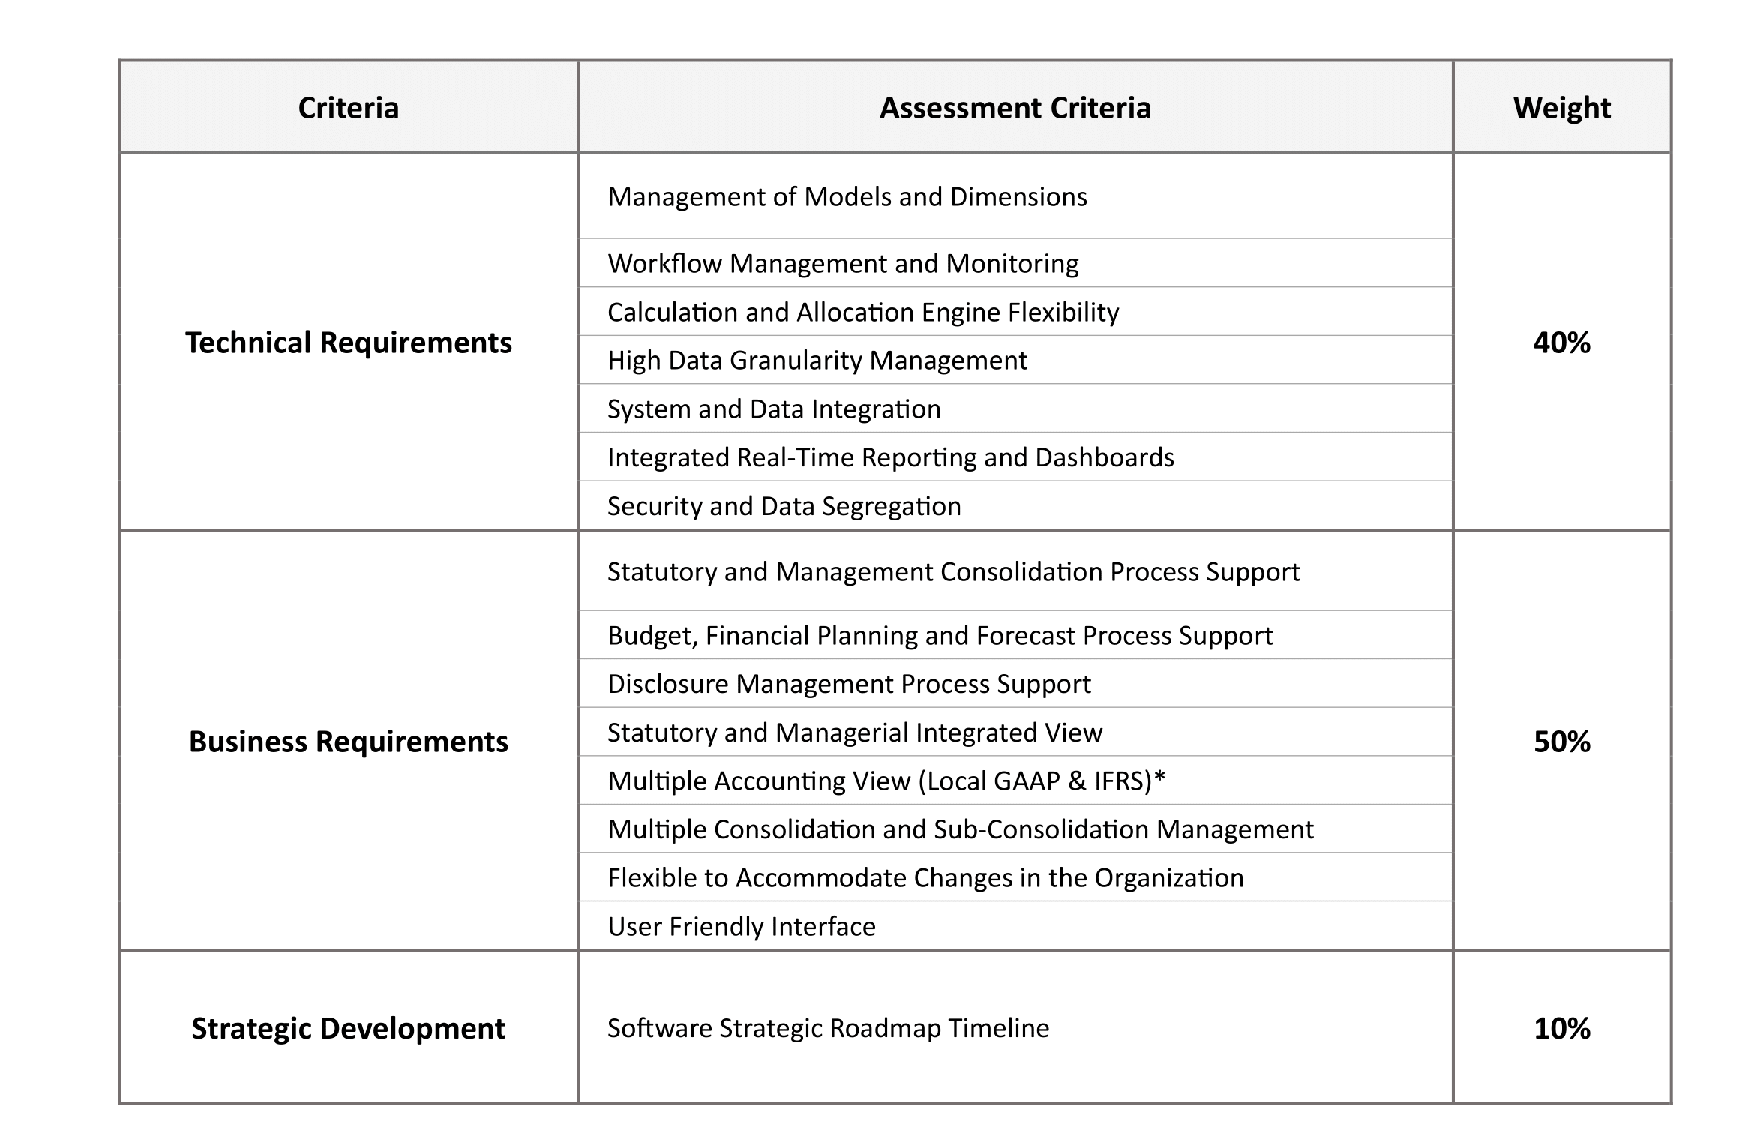
\includegraphics[width=\linewidth]{figures/requirements.pdf}
	\caption{Technical, Business and Strategic Requirements}
    \floatfoot{*Generally Accepted Accounting Principles (GAAP) and International Financial Reporting Standards (IFRS)}
	\label{fig:requirements}
\end{figure}

Figure \ref{fig:requirements} lists all the technical, business and strategic requirements that should be considered when choosing the right tools and technologies for the implementation of the EPM solution.
%
It is important to identify and prioritize both business requirements and technical requirements when planning an EPM implementation project, in order to build an effective and maintainable solution.

Technical requirements cover the specific features and capabilities that the system must have in order to ensure that the EPM system is effective, reliable, and able to meet the unique needs of the Group and its entities.
%
More in details, the use of technologies that allow for integrated modeling that is easy-to-maintain and with no limitations of dimensions is of key importance for this project.

For example, a Holding Group which owns different Brands and entities across the globe may need to frequently update the \textit{Product} or \textit{Geography} dimension every time they add a new product or sell to a new country.
%
At the same time, users need to have a clear and structured workflow of activities that supports them in the use of the EPM system, while the Control Group should be able to track and monitor the progress of single activities carried out by the entities.

Then, in terms of calculation and allocation flexibility, we refer to the possibility to perform custom calculations and extend predefined rules (like consolidation and currency translation), in order to meet the specific needs and requirements of each entity.
%
The system should also be able to manage data of different granularity as the level of detail and precision in data structures depends on the activity to perform.
%
The EPM platform needs to manage high-volume data and possibly interface with big data systems.

Naturally, system and data integration must be available.
%
In particular, the system should have an integrated solution for ETL (Extract, Transform and Load) activities, completed with advanced mapping features to accommodate multi-source and multi-ERP loading.

Reporting and dashboarding can be setup ``live'' for all data available in the interconnected solution
applications to enable the Group to make informed decisions based on its financial data.

Finally, the EPM system should have robust security features to protect sensitive financial data, while allowing the Control Group to manage granular securities at the micro-detail of data to handle the read and write permissions of the different entities.

Business requirements, on the other hand, regard the specific goals, needs, and expectations of the stakeholders and users of a system. 
%
In our context of EPM implementation project for a Holding Group, business requirements are set to reach key business goals, like streamlining financial reporting, improving decision-making based on financial data, increasing efficiency and accuracy in budgeting and forecasting, and providing a centralized system for financial management across all entities. 

One of the key priorities for a Holding Group is to have a clear statutory and consolidation process with the possibility to adopt multiple consolidation methods, including full consolidation, proportionate consolidation, and equity consolidation.
%
Consolidation accounting is the process of combining the financial results of several subsidiary companies into the combined financial results of the parent company as though they were a single firm.

The system should have predefined modules to address different planning standard processes and an open ``free from'' planning mode to create personalized planning environments. 
%
At the same time, it should include embedded predictive planning, risk based planning and strategic  long-term modeling feature.

Public companies must prepare disclosure reports for internal and external stakeholders to shine a light on the company's performance and operating activities.
%
Disclosure reports contain information about a company's business activities, financial condition, management compensation, operating performance and future direction. 
%
It is therefore essential for the EPM system to provide disclosure management functionalities to help the Group to fulfill the disclosure requirements of regulators like the Security and Exchange Commission or the European Central Bank.

The system should provide  a unified environment able to guarantee the consistency and coherence of data generated at each level of the statutory, management and disclosure reporting.
%
In this regard, users should be able to compare multiple accounting views depending on the country of interest (GAAP for United States and IFRS world-wide).

Finally, the EPM system should be flexible enough to adapt to changing business needs and requirements, allowing for an easy-to-use, adjustable interface that every user can use to create different versions of reports, depending on the current need.

At the strategic level, making architecture changes or modifying operations takes a clear plan of where the organization is, where it wants to go, and how to get there. 
%
A strategic road-map lays out the direction of IT efforts that span across an organization in a simple way to align teams and key stakeholders.
%
The implementation of the EPM solution should be in line with the company's strategic road-map, both in terms of deliverables, process schedule and timing.

%----------------------------------------------------------------------------------------
\chapter{Case Study: Oracle Cloud Implementation}
\label{chap:implementation}
%----------------------------------------------------------------------------------------

In this chapter we will explore the case study of an Oracle Cloud EPM implementation project for an international Group with multiple entities.
%
Such implementation was necessary for the Group to streamline financial reporting, improve decision-making based on financial data, and, most importantly, provide a centralized system for financial management across all entities.

The Group has a complex financial structure and was facing significant challenges in managing financial data across all entities. 
%
Its financial systems were disconnected, making it difficult to get a clear view of financial performance and to generate accurate and timely reports. 
%
In addition, the Group's reporting processes were inefficient, relying heavily on manual data entry and resulting in errors and inconsistencies. 
%
Also, they lacked visibility into financial data across all entities, making it difficult to make informed decisions and to drive growth and profitability.

Throughout this case study, we will examine the challenges faced during the implementation process, the solutions that were implemented, and the outcomes of the project.
%
We will start by defining the challenge, then we will explore the solution selection process and examine in depth the implementation phase.

\section{EPM solution selection}

Selecting the right EPM solution is crucial to effectively manage the financial data of the Group and drive growth.
%
In order to design a solution architecture for consolidation, planning and reporting that is able to provide system integration, automatic and standard processes, we need to identify the most suitable EPM tool among the ones available in the market.

\begin{figure}[htbp]
	\centering
	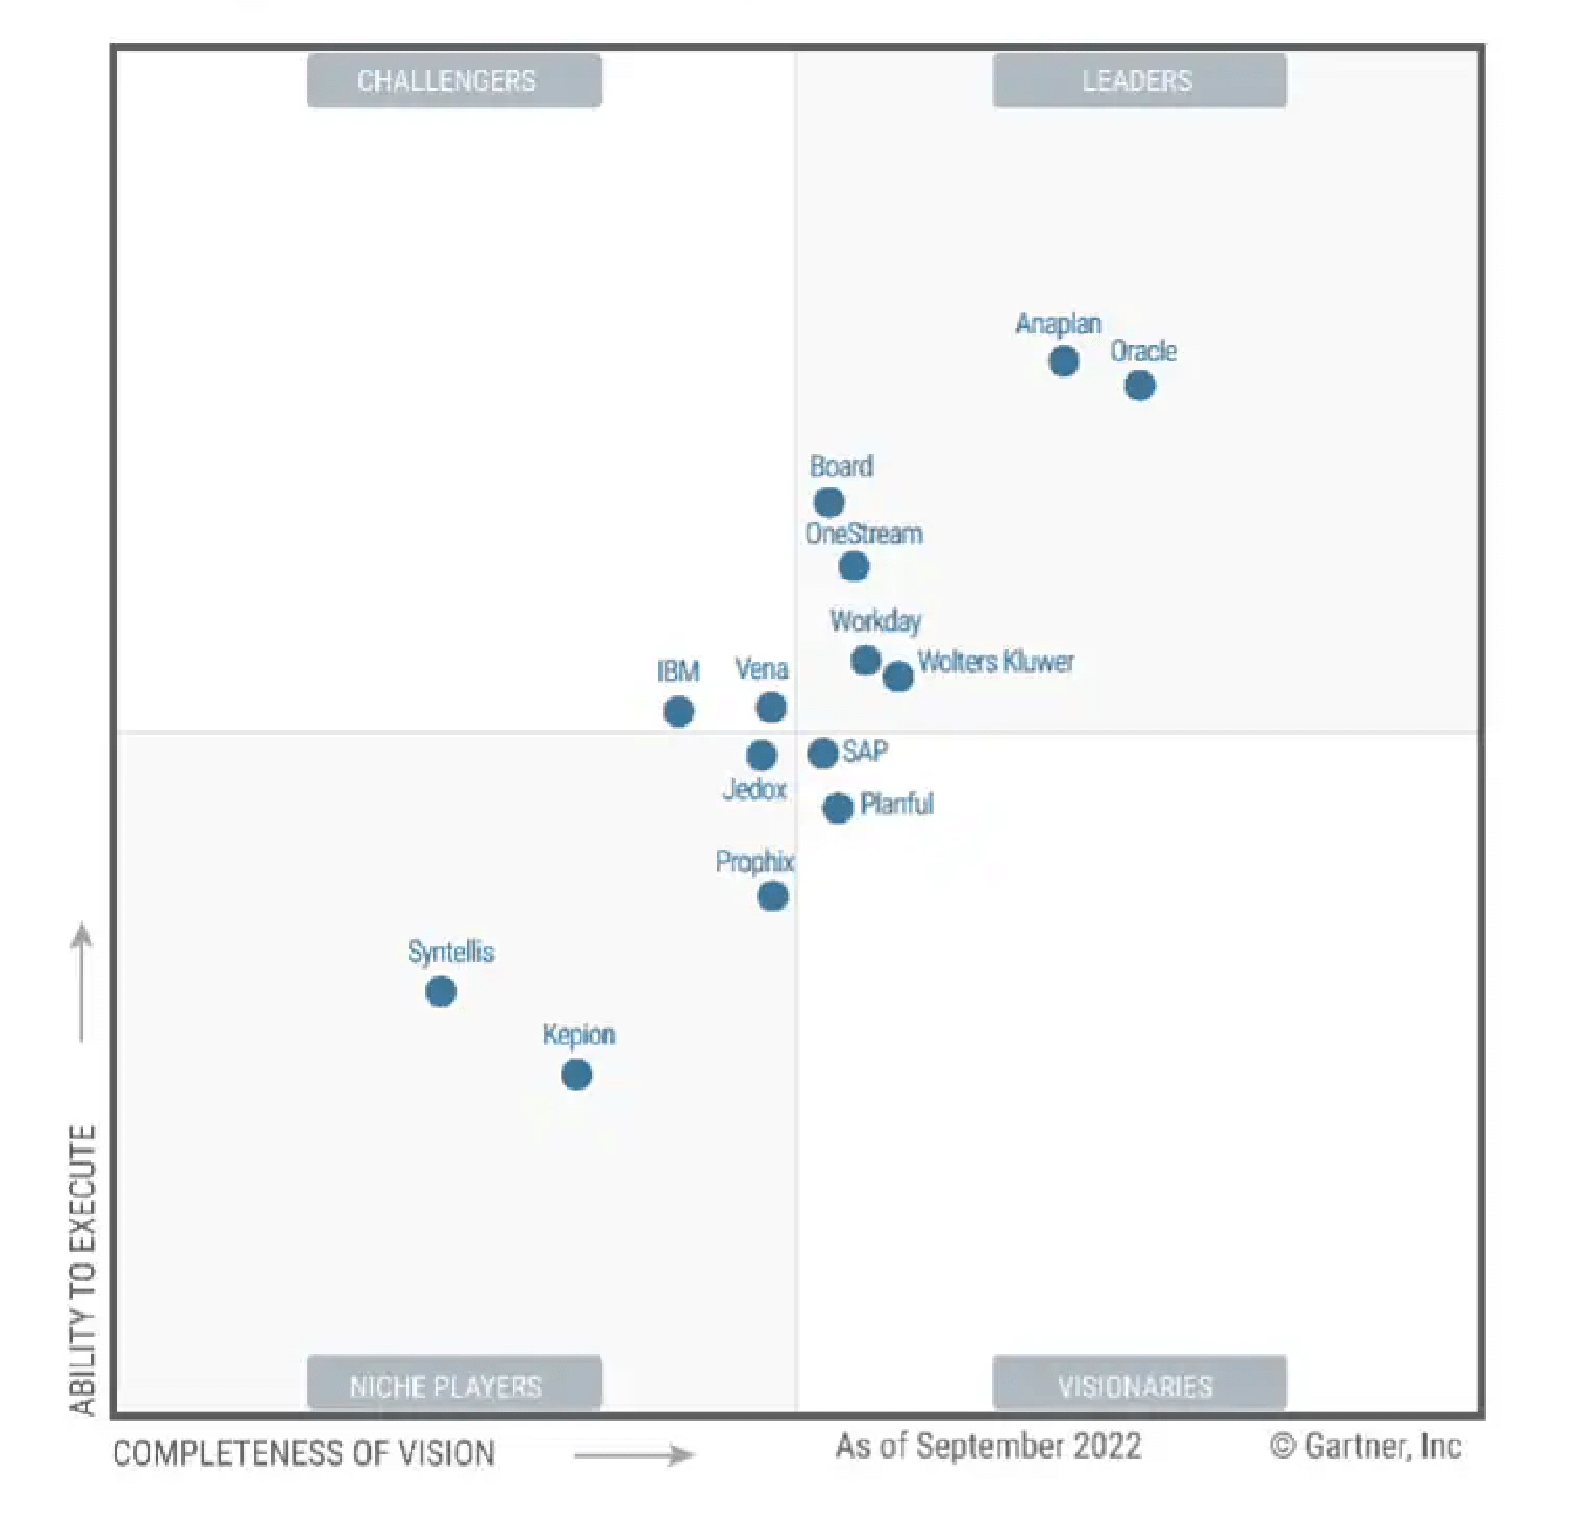
\includegraphics[width=\linewidth]{figures/gartner.pdf}
	\caption{Magic Quadrant for Financial Planning Software}
    \floatfoot{Source: Gartner (December 2022)}
	\label{fig:gartner}
\end{figure}

Figure \ref{fig:gartner} displays the Gartner Magic Quadrant for financial planning software published on the 14th December, 2022 \cite{gartner2022magic}.
%
Gartner defines Financial Planning Software as ``the key tool that enables organizations to manage their enterprise-wide financial planning, forecasting, and budgeting processes.'' \footnote{Gartner is a registered trademark and service mark and Magic Quadrant is a registered trademark of Gartner, Inc. and/or its affiliates in the U.S. and internationally and are used herein with permission. All rights reserved.}

Financial Planning Software solutions allow organizations to plan and analyze the business financial strategy across all three financial statements (profit and loss, balance sheet, and cash flows). 
%
It supports modeling, collaboration, analytics, and performance-reporting capabilities, all of which enhance a user’s ability to effectively manage financial performance.

The Magic Quadrant evaluates vendors based on their completeness of vision and ability to execute. 
%
Oracle Cloud has been named a Leader in the Gartner Magic Quadrant for Cloud Financial Planning and Analysis Solutions for several years in a row. 
%
This recognition highlights Oracle's continued commitment to innovation and customer satisfaction. 
%
As a Leader in the Magic Quadrant, Oracle Cloud is recognized for its ability to provide a comprehensive and customizable EPM solution for holding Groups and other organizations.

According to Oracle Corporation, the current global uncertainties have proven the value of Oracle Fusion Cloud EPM as businesses of every size have experienced extreme volatility in demand and supply environments, making agility in financial planning processes a must-have competency \cite{toomey2022oracle}.

The ability to support and connect planning across the organization is a competitive differentiator. 
%
Oracle delivers purpose-built solutions to streamline and manage planning processes in sales, marketing, human resources, IT and supply chain functions.

Oracle Cloud EPM brings together multiple Enterprise Performance Management capabilities into a single suite: financial and operational planning, profitability and cost management, account reconciliation, consolidation and close, tax reporting, narrative reporting, and enterprise master data management. 
%
These capabilities, along with built-in best practices, help customers to gain value quickly.

For the Holding Group in our case study, Oracle Cloud EPM was the right choice due to its ability to be customized to meet the specific needs of the organization, its comprehensive security and compliance features, and its strong support and training resources.
%
Choosing the right EPM solution can make all the difference in the Group's ability to effectively manage their financial data and drive growth and profitability.

\section{Elements of the implementation process}

To successfully implement a new system, it is essential to have a comprehensive understanding of the various elements that are involved in the process. 
%
This section explores the essential elements necessary for a successful EPM implementation process, providing a roadmap for organizations seeking to deploy EPM solutions effectively.
%
Throughout this section, we will delve into key components that form the foundation of an EPM implementation solution. 
%
At the same time, we will provide practical insights, best practices, and real-world examples specific to the case study, to better explain the steps to undertake and the variables to consider when implementing and EPM solution.

\paragraph{License}

Oracle Cloud Enterprise Performance Management is a complete and connected EPM solution which, with one licensing subscription, gives access to planning, close and consolidation, account reconciliation, narrative reporting, and more.
%
Users can access all these models with their license; they do not need a license for each model.
%
There are two types of licenses according to which specific functionalities and features for users are enabled within the application:
%
The user-based licenses are assigned to individual users who require access to the application.
%
These licenses provide access to specific functionalities within the application, and the features available to each user may vary based on the license type and configuration.
%
On the other hand, instance-based licenses are allocated to the overall EPM environment, rather than individual users. 
%
These licenses are typically purchased in bundles and may be allocated based on factors such as the number of users or the level of usage.

Oracle will provision by default two environments to users: one environment dedicated to production use and a second environment dedicated as a staging environment for non-production use.
%
Additional environments or business processes can be ordered and provisioned separately.

\paragraph{Environments}

Oracle Cloud EPM applications are typically deployed in two environments: production and test.
%
The production environment is the live environment where users interact with the EPM application to perform their day-to-day financial management tasks.
%
The test environment, on the other hand, is a sandbox environment in which we can test new features, perform system upgrades, and make changes without affecting the live production environment. \\

\begin{lstlisting}
https://epm-[test]-idDomain.epm.dataCenterRegion.oraclecloud.com/epmcloud
\end{lstlisting}

Both the environments can be accessed via unique launch URLs composed by the service name (EPM), the type of environment (test or production), the identity domain name and the data center in which the environment is located.

\paragraph{Modules and Applications}

The suite of Oracle Cloud EPM includes various modules that are designed to address specific business needs:
%
Planning and Budgeting enables organizations to streamline their budgeting and forecasting processes, allowing for collaboration across teams, flexible modeling, and real-time updates to data.
%
Financial Consolidation and Close automates the financial consolidation and close process, helping organizations to reduce errors and improve accuracy, providing a standardized approach to the close process and supporting compliance with regulatory requirements.
%
Account Reconciliation streamlines the account reconciliation process, helping organizations to reduce risk and improve accuracy. 
%
Profitability and Cost Management enables organizations to gain insights into their profitability and cost structures, supporting activity-based costing, providing allocation and modeling capabilities and what-if analysis.
%
Enterprise Data Management provides a centralized platform for managing master data across the organization, supporting data governance and compliance, data quality management capabilities, and enabling seamless integration with other EPM modules.
%
Narrative Reporting enables organizations to create, manage, and distribute financial and management reports.
%
Tax Reporting supports compliance with tax regulations and provides a comprehensive solution for tax reporting, including a tax data warehouse, data validation and mapping capabilities, and supporting data visualization.
%
In this case study, we will see more in details the Planning and Budgeting application together with Oracle's Financial Consolidation and Close Solution (FCCS) and Enterprise Data Management.

\paragraph{Data Structure}

One of the core components of Oracle Cloud EPM is Essbase, which is multidimensional database management system (MDBMS) that enables businesses to store, manage, and analyze large volumes of data from different sources.
%
Multidimensional databases are specialized databases designed for online analytical processing (OLAP). 
%
They store data in a cube-like structure where each cell represents a specific data point.
%
Unlike relational databases, which store data in tables, multidimensional databases use a multidimensional model that allows users to analyze data across multiple dimensions, such as time, geography, and product. 
%
One of the key features of MDBs is their ability to perform OLAP, enabling users to drill down or roll up data along different dimensions, providing a more comprehensive view of the data. 
%
Compared to Relational Databases, multidimensional Databases are faster and more efficient when dealing with large volumes of data, even though they are less flexible than RDBs when it comes to data modeling, and require specialized tools and expertise to manage and maintain.

\paragraph{Data Management}

Data management refers to the process of integrating and managing data from various sources within the EPM environment. 
%
The process begins with integrating data from various sources, such as ERP systems, spreadsheets, or other databases. 
%
Oracle Cloud EPM provides tools to help users extract and integrate data from these sources and map them to the appropriate EPM application or service.
%
Once the data has been integrated into the EPM environment, it needs to be validated to ensure that it is accurate, complete, and consistent. 
%
After the data has been validated, it may need to be transformed to match the specific requirements of the EPM application or service using predefined mappings, calculations or custom scripts.
%
Finally, the data can be loaded into the EPM application into the appropriate data structures within the application, such as dimensions or cubes. 
%
Oracle Cloud EPM provides tools to automate the steps of data management,  helping organizations streamline their data management processes allowing for a faster data integration with improved data quality, greater efficiency and reduced error rate.

\paragraph{Dimensions}

In Oracle Cloud EPM, dimensions are a fundamental component of multidimensional data modeling. 
%
Dimensions provide a way to organize and analyze data in a multidimensional structure, allowing users to perform complex analysis along them. 
%
They are typically structured as hierarchies, with each level in the hierarchy representing a different level of detail. 
%
Members represent the values within each level of the hierarchy and can be associated with attributes such as descriptions or tags to provide additional context. 

Hierarchies provide the ability to roll up or drill down data to gain insights into different levels of detail. 
%
Through dimensions, it is possible to execute dynamic calculations to generate on-the-fly calculations at runtime, without requiring the user to manually enter the data. 
%
This enables users to create dynamic models that are more flexible and responsive to changing business needs.

As we can see in figure \ref{fig:hierarchy}, the time dimension follows a tree-like structure where each level in the hierarchy represents a different level of detail. 
%
Hierarchies allow users to organize data into a structure that is easy to understand and navigate it, by grouping related data points together and providing a way to analyze data at different levels of detail, from high-level summaries to more detailed views of individual data points.
%
In this dimension, data can be dynamically aggregated along the levels in order to see the results with different levels of granularity, i.e. monthly, quarterly or yearly.

\begin{figure}[htbp]
	\centering
	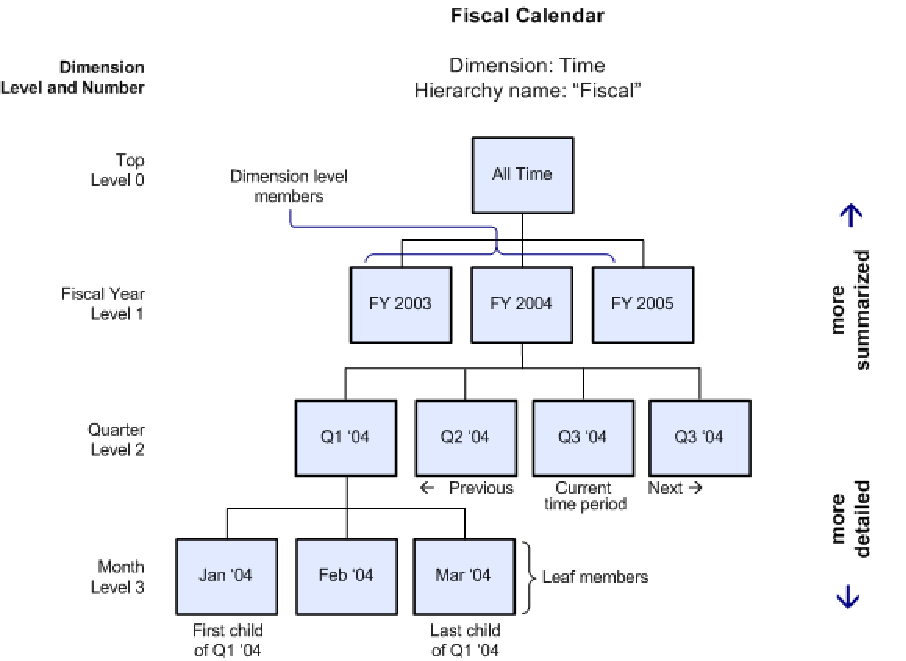
\includegraphics[width=\linewidth]{figures/hierarchy.pdf}
	\caption{Hierarchical Structure of the Time Dimension}
    \floatfoot{Source: Oracle User's Guide}
	\label{fig:hierarchy}
\end{figure}

\paragraph{Forms and Reports}

Forms and reports are key components of Oracle Cloud EPM that enable users to interact with and analyze data in a multidimensional database. 
%
Forms are used to input or edit data, while reports are used to analyze data in a structured format.

Forms provide users with a familiar interface for entering or editing data in a multidimensional database. 
%
They can be designed to incorporate a variety of data entry methods, including text boxes, drop-down lists, and radio buttons. 
%
Users can also navigate between different cells and dimensions in a form to enter or edit data in a specific location.

Reports, on the other hand, provide a way to analyze data in a structured format. 
%
These reports can be customized to include specific data points and dimensions, and can be designed to incorporate a variety of formatting options, including charts, graphs, and tables.

One of the key advantages of forms and reports is their flexibility. 
%
Users can design and customize forms and reports to meet their organization's unique business requirements, incorporating specific data points and dimensions as needed. 
%
This makes forms and reports a powerful tool for data analysis and decision-making.

\paragraph{Business Rules}

Business rules are a set of instructions that define how data should be calculated or transformed in a multidimensional database. 
%
These rules are used to automate complex calculations, validations, and transformations in a data model, reducing the need for manual data entry and increasing the accuracy of data analysis.
%
Business rules can be created using the Calculation Manager, which is the tool used to create, validate, deploy, and launch calculations in Oracle Cloud EPM. 
%
These rules can be based on various input data sources, including data entered manually, data loaded from external sources, or data calculated dynamically using other rules.
%
One of the key advantages of business rules is their flexibility: users can define rules that incorporate complex logic and are specific to their organization's unique business requirements. 
%
Rules can also be modified or updated easily as business needs change, making them a dynamic tool for data analysis.
%
%Oracle Planning offers powerful calculation features, including support for complex formulas, allocation rules, drivers, and multidimensional calculations. This enables organizations to perform sophisticated calculations while maintaining flexibility in their planning processes.


\paragraph{Smart View}

Smart View is an Excel add-in that allows users to connect to and interact with data in Oracle Cloud EPM. 
%
With Smart View, users can access dimensions, forms and reports directly from within Excel, enabling them to analyze and manipulate data in a familiar interface.
%
One of the key advantages of Smart View is its ability to integrate seamlessly with Excel. 
%
Users can work with data in Excel as they normally would, but with the added ability to access and manipulate data in a multidimensional database. 
%
This enables users to perform complex calculations and data analysis tasks using Excel's built-in functionality.
%
Smart View also provides a wide range of functionality beyond basic data access and manipulation. 
%
For example, users can use Smart View to create and manage ad-hoc reports, design custom templates for data entry and analysis, and build complex financial models using Excel's built-in functionality.
%
Another key advantage of Smart View is its ability to work with multiple data sources. 
%
Users can connect to and analyze data from a variety of sources, including Planning and Budgeting, Financial Close and Consolidation and more. 

\section{Building a comprehensive EPM solution}

The implementation of this EPM solution involves a systematic and comprehensive process which is aimed at ensuring accurate and comprehensive reporting to the user.
%
One crucial aspect of this process regards the creation of the dimensions that will be used to build reports from various perspectives. 
%
They are used to categorize and structure information in order to obtain a complete view on the performance of the Group.

Dimensions are the building blocks of an EPM system; they serve as the axes along which data is organized and analyzed, providing a multidimensional view on financial and operational information. 
%
Each dimension consists of a hierarchical structure which allows users to drill down information from high-level summaries to more granular details and vice versa.

Dimensions serve several purposes, including analysis and reporting, data integration and restructuring.
%
First of all, dimensions allow for the segmentation and grouping of data which facilitate analysis and reporting by enabling users to generate reports based on specific dimensions, providing insights from different angles.
%
At the same time, they act as a common framework for integrating data from various sources within the Holding Group. 
%
Specifically, by aligning different systems and processes with a consistent set of dimensions, data can be harmonized and consolidated for accurate analysis and reporting.
%
Finally, dimensions provide flexibility to adapt to changing business requirements as they can be modified, expanded, or restructured to accommodate new entities, geographies, products, or brands as the Group evolves.

Building dimensions require a systematic process during which different aspects are taken into account.
%
The first step is to analyze the specific needs of the Group to identify the dimensions that will provide meaningful insights for analysis and reporting.
%
Then, it is essential to determine the levels of the hierarchy for each dimension and assign member properties to capture additional information about each dimension member. 
%
These properties provide contextual information and can include attributes such as currency, time zone, brand category, or legal entity type. \\

\begin{figure}[htbp]
	\centering
	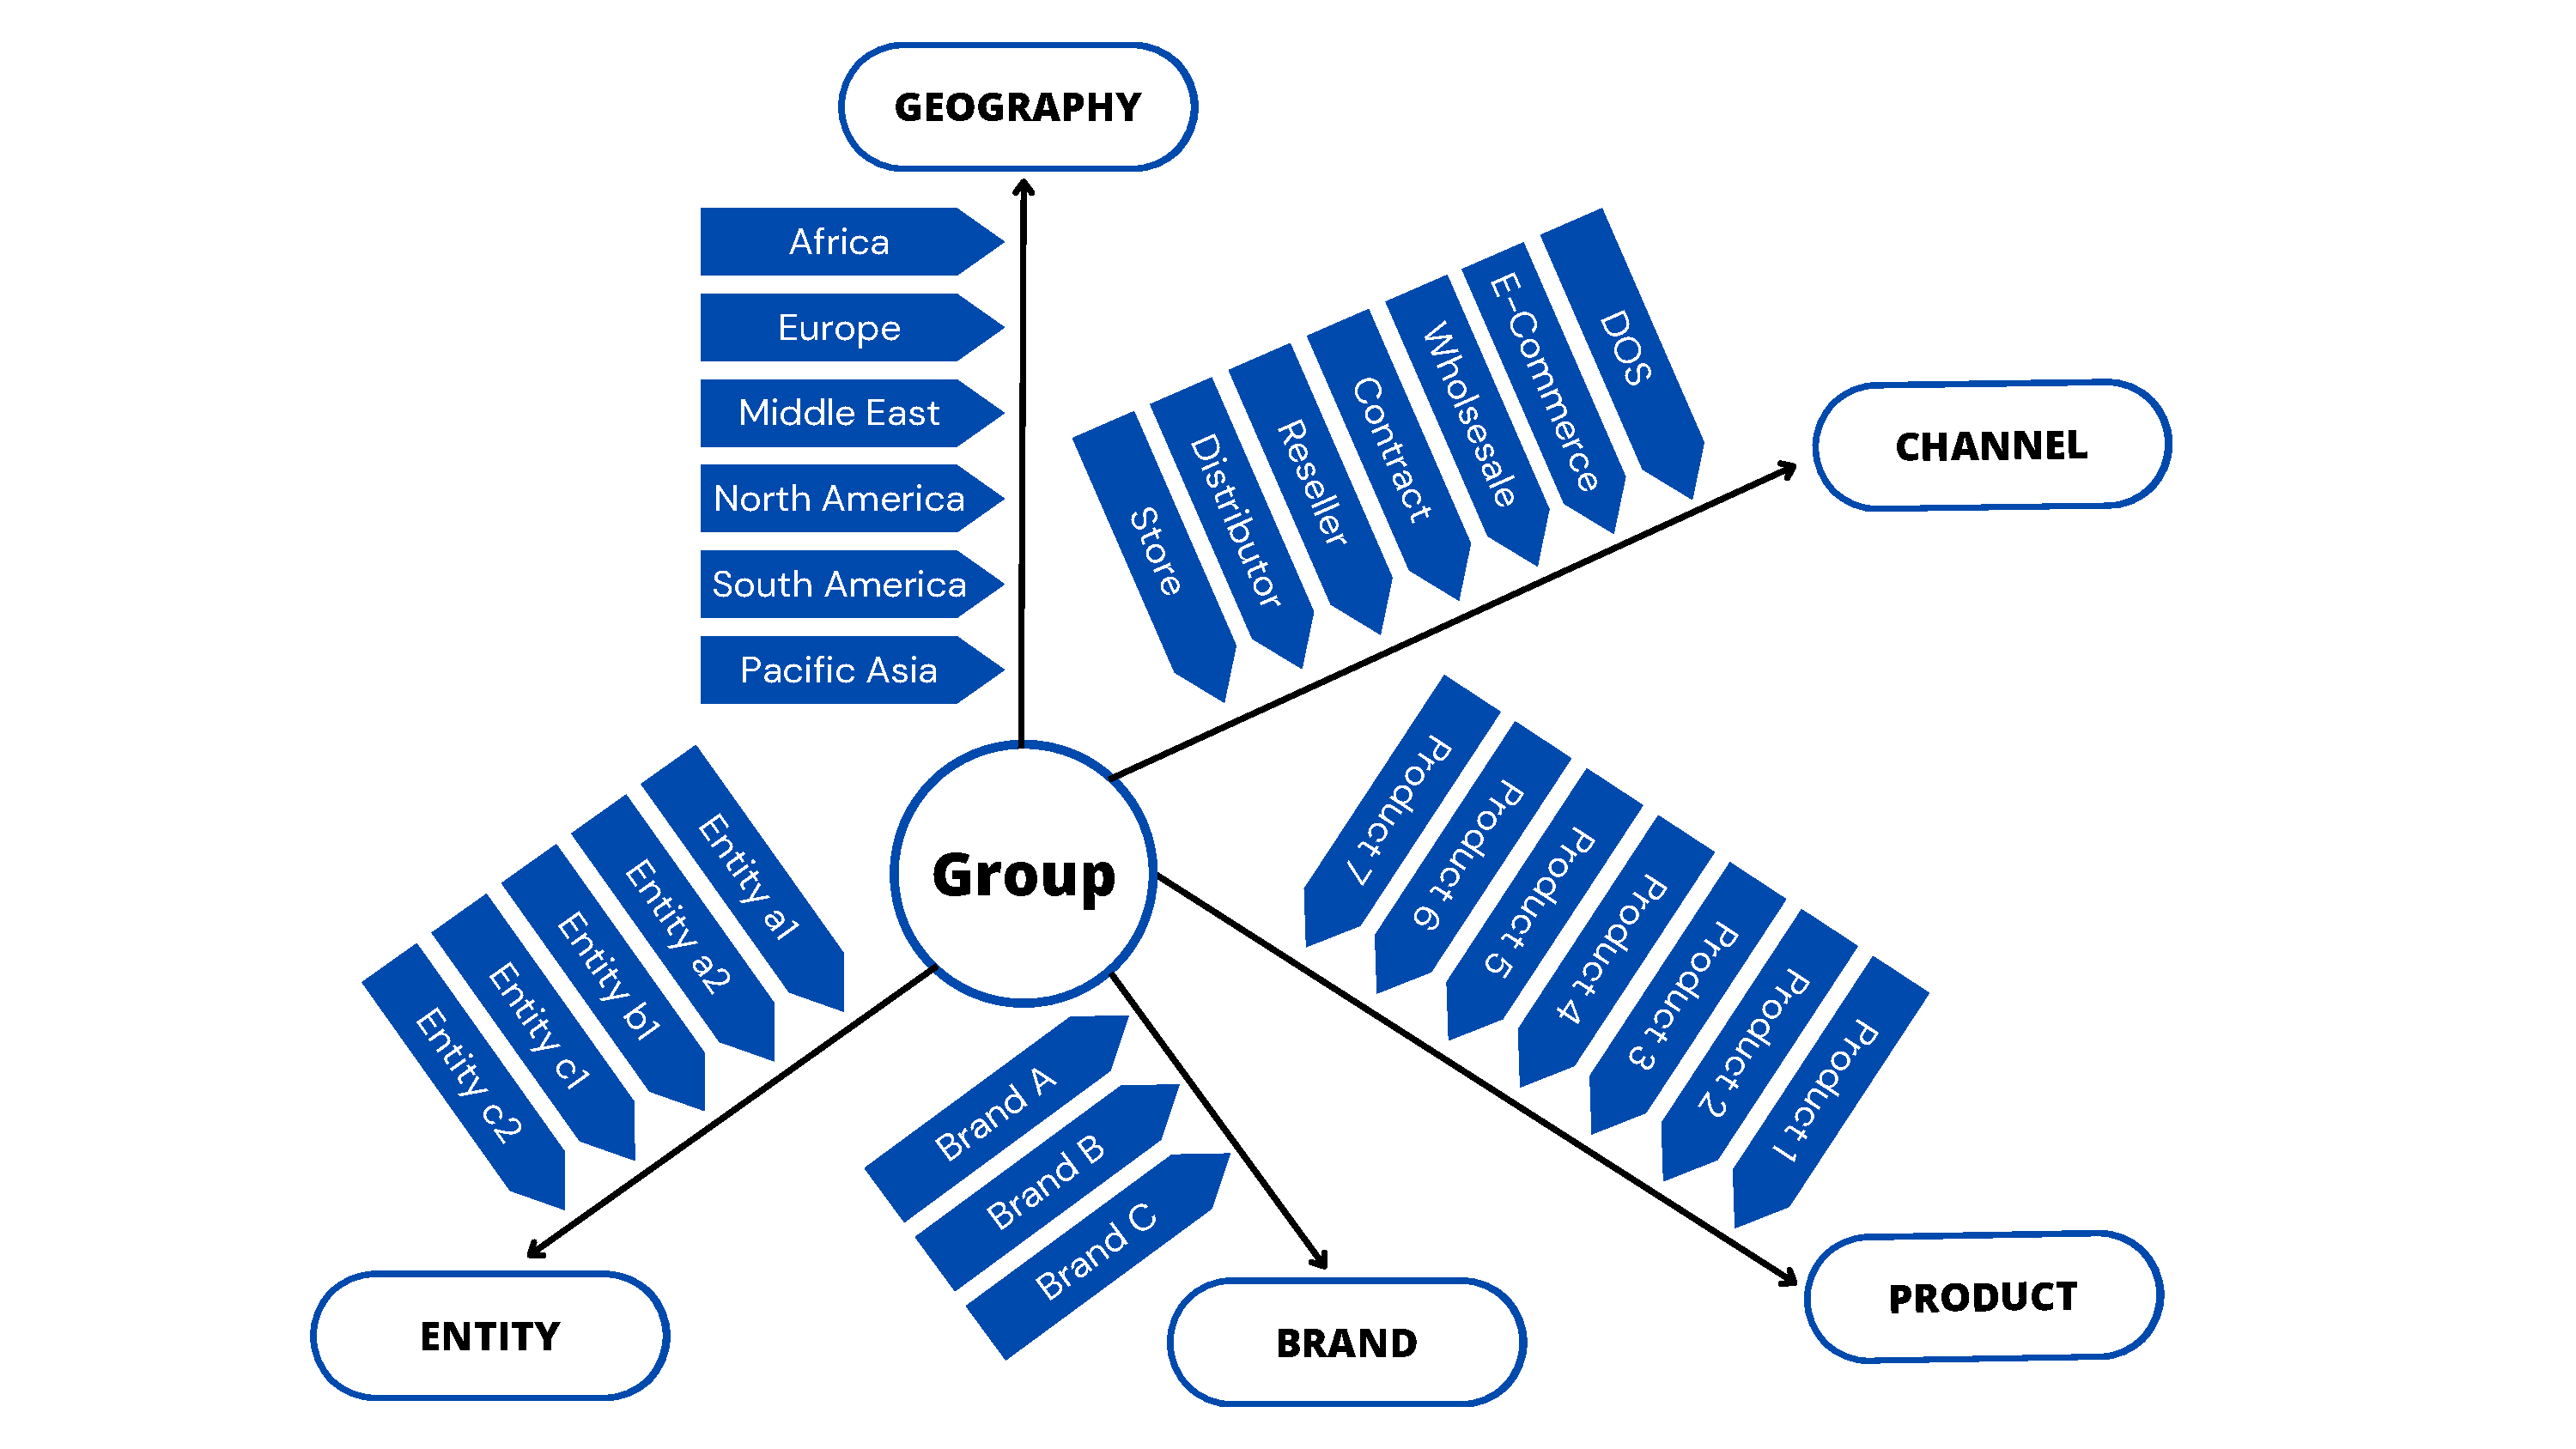
\includegraphics[width=\linewidth]{figures/dimensions.pdf}
	\caption{Dimensions of Analysis}
	\label{fig:dimensions}
\end{figure}

As we can see in figure \ref{fig:dimensions}, the activities of the group will be evaluated under five different dimensions of analysis: geography, channel, product, brand and entity.
%
The geography dimension helps analyze financial and operational data based on different geographic regions, thus enabling the Holding Group to understand the performance of its entities across different countries, states, or regions. 
%
The first step to implement such dimension is to determine the levels of geography that are relevant for the analysis, such as country, state, city, or region.
%
Here, the geography dimension include three main geographical groups - EMEA (Europe, Middle East, Africa), Americas and APAC (Asia-Pacific) - which are further subdivided in smaller areas like Middle East, Nordics, Greater China and others.
%
The product dimension allows for a detailed analysis of revenue, costs, and profitability across various product lines, enabling users to analyze data and get insights based on different products.
%
The brand dimension enables analysis and reporting based on different brands owned or managed by the Holding Group. It helps assess brand performance, market share, and customer preferences.
%
The entity dimension allows for analysis and reporting based on individual entities within the Holding Group, allowing the assessment of the performance of each entity separately and in comparison within each others.
%
Finally, the channel dimension allows for analysis based on different distribution channels used by the companies to deliver the products and helps assess sales performance and customer preferences across the various channels. 

Once dimensions have been defined, the next crucial step is to load and map the data within the EPM solution and, more in details, to the Financial Consolidation and Close Solution (FCCS). 
%
To populate the dimensions with data, the Holding Group needs to collect financial data from all the entities of the Group as illustrated in figure \ref{fig:dataload}.
%
Of course, different entities have different data collection tools and methodologies, ranging from ERP software solutions, Excel spreadsheets, BI tools or cloud solutions.
%
Each Brand is responsible for collecting the financial data of entities that belong to it, which will be transformed and adapted in order to meet the standards for loading.  
%
FCCS allows users to integrate financial data from various sources, such as ERP systems, spreadsheets, and other data sources by means of pre-built connectors that allow users to easily integrate data.

Connectors are software components that enable different applications or systems to communicate and exchange data with each other. 
%
They act as intermediaries, allowing data to flow between two different systems that may use different data formats or data protocols.
%
In FCCS, connectors provide a standardized interface for connecting different systems for integrating data, allowing them to communicate using a specific data format and protocol.

\begin{figure}[ht]
	\centering
	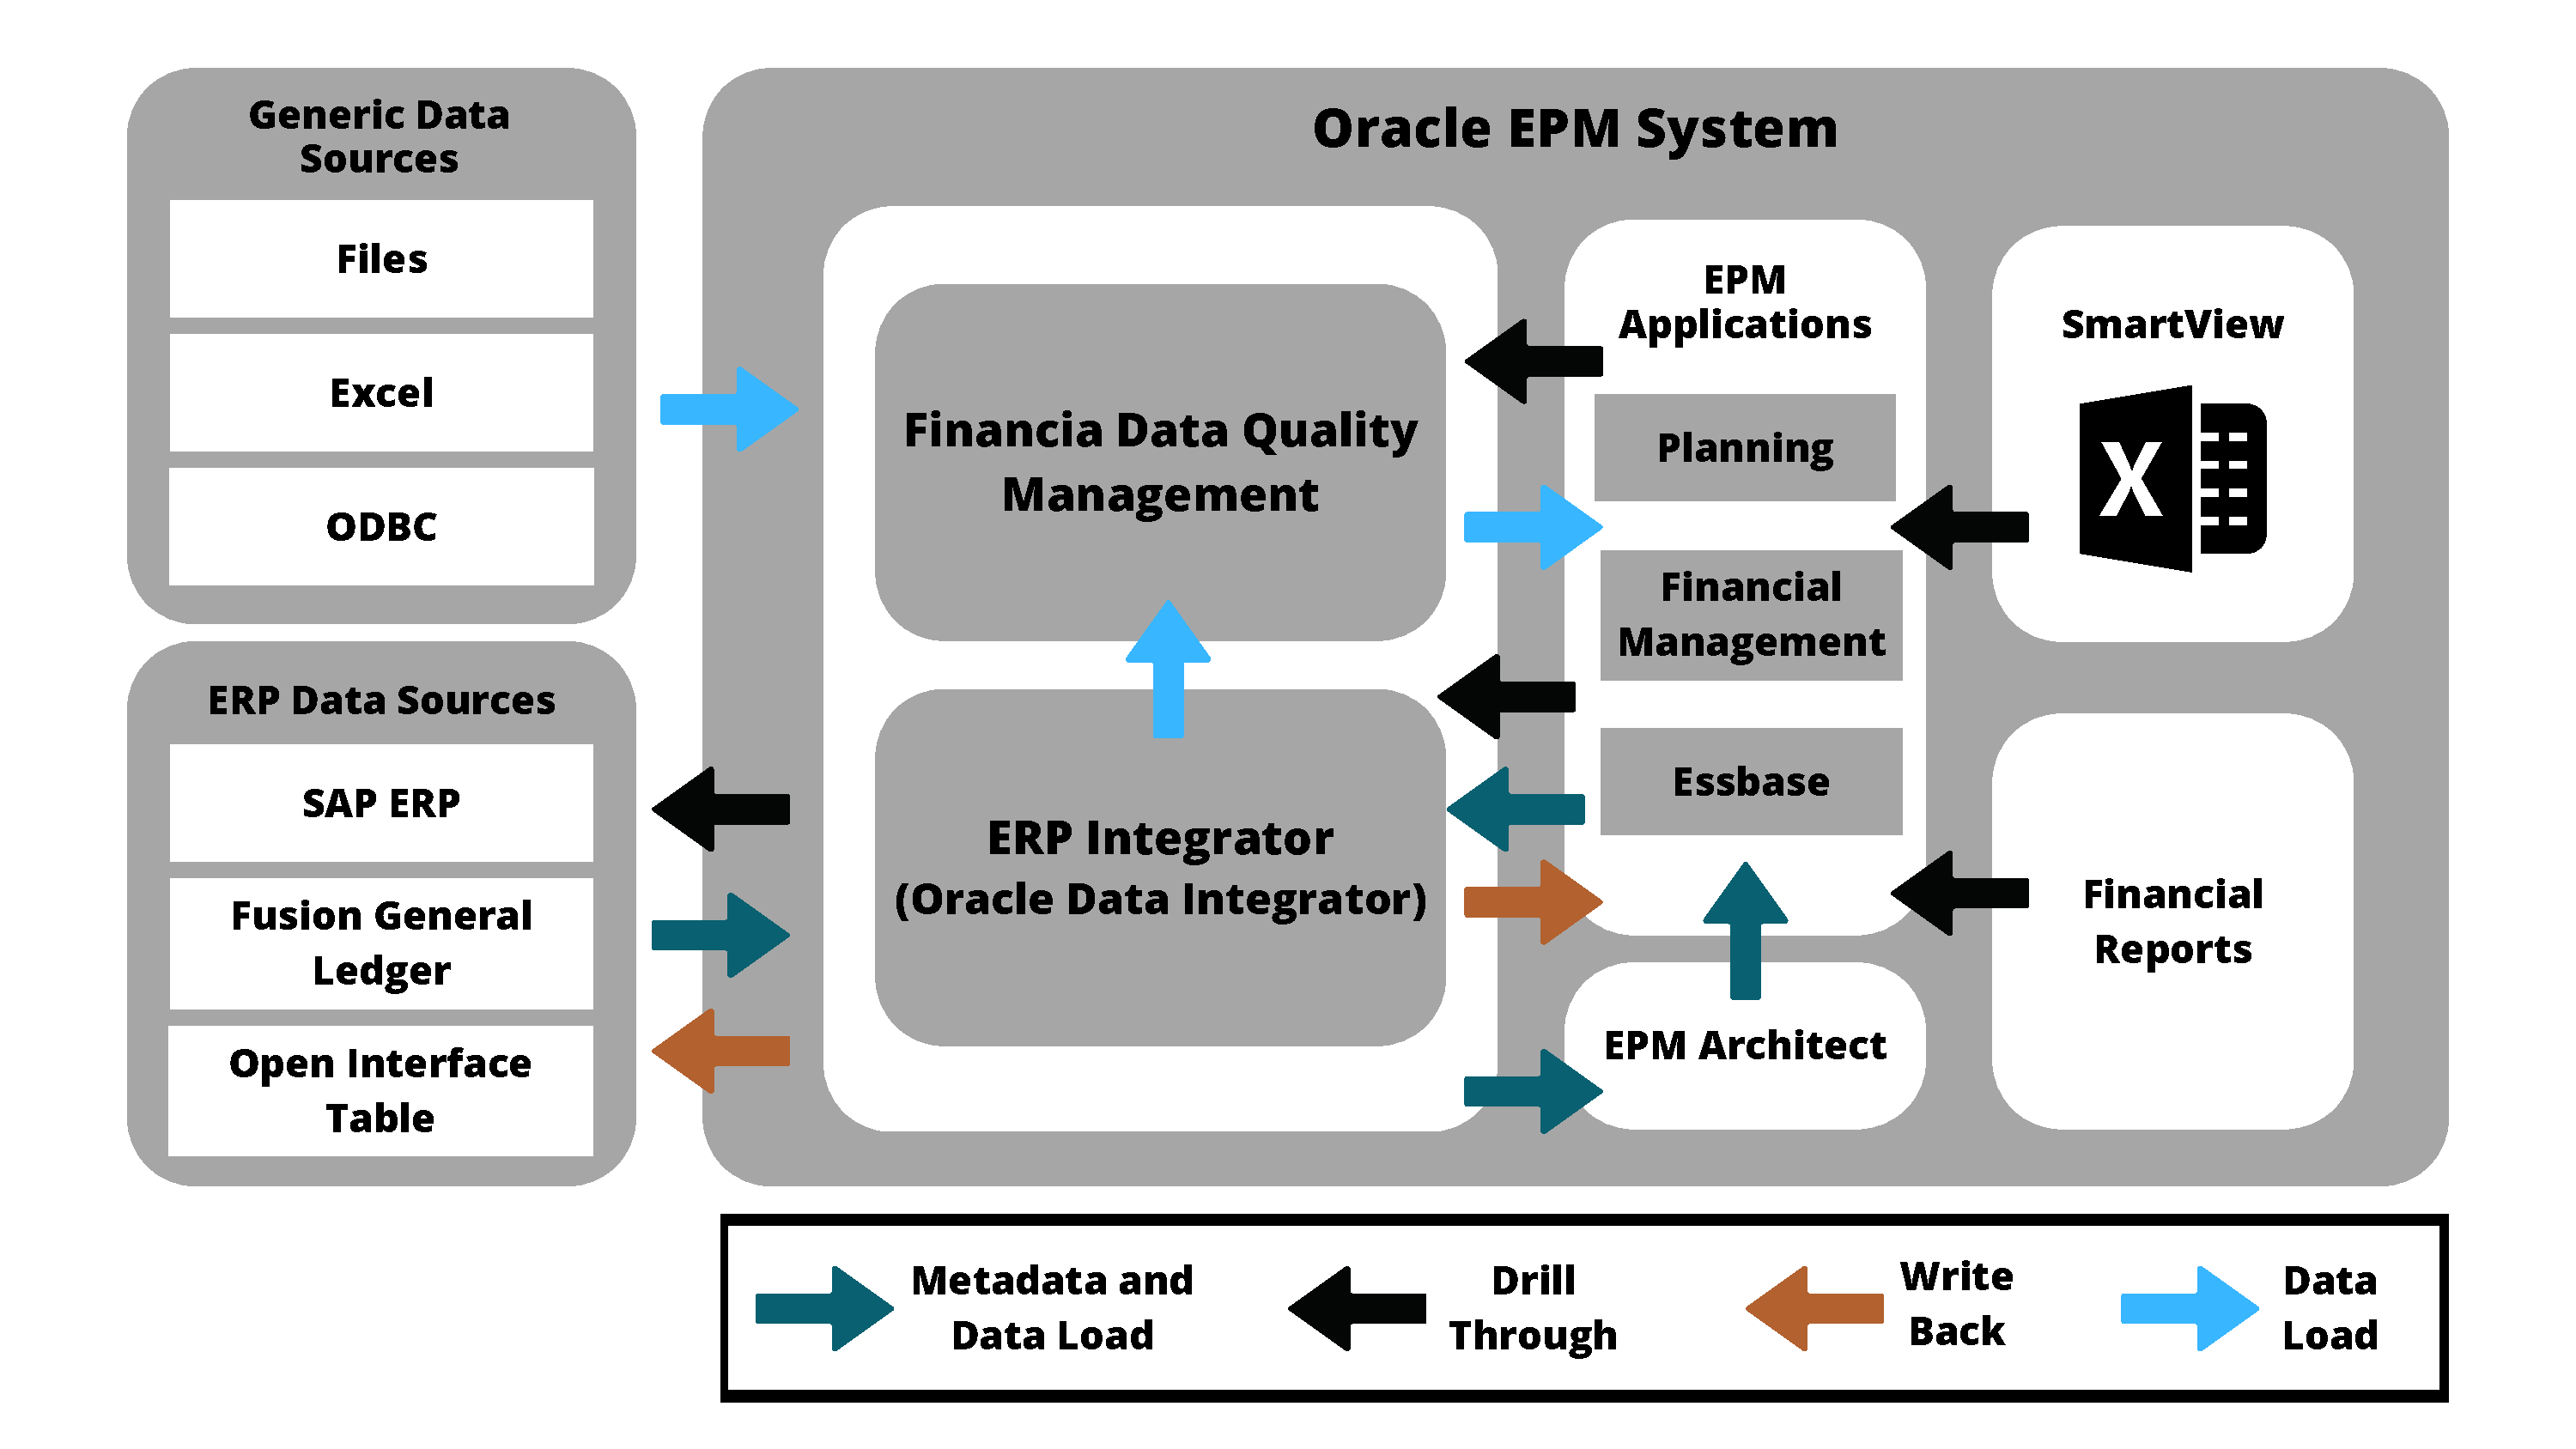
\includegraphics[width=\linewidth]{figures/data-load.pdf}
	\caption{Data Collection Process Across the EPM System}
    \floatfoot{Source: Oracle User's Guide} 
	\label{fig:dataload}
\end{figure}

At the same time, FCCS allows users to map data from different sources to the appropriate dimensions and members, thus ensuring that data is correctly integrated and consolidated even if it comes from different systems with different structures.
%
Data mapping refers to the process of aligning data from different source systems to the dimensions and members in a target system.
%
It involves identifying the relevant data elements in the source system, and then mapping them to the appropriate dimensions and members in the target system. 
%
This process requires an understanding of the data structures and formats used in the source and target systems, as well as the business logic and rules governing the mapping process.
%
Effective data mapping is critical for ensuring the accuracy and completeness of data integration and migration processes; if data is not mapped correctly, it may be lost, duplicated, or incorrectly integrated, resulting in errors and inconsistencies in the target system. 

\begin{figure}[htbp]
	\centering
	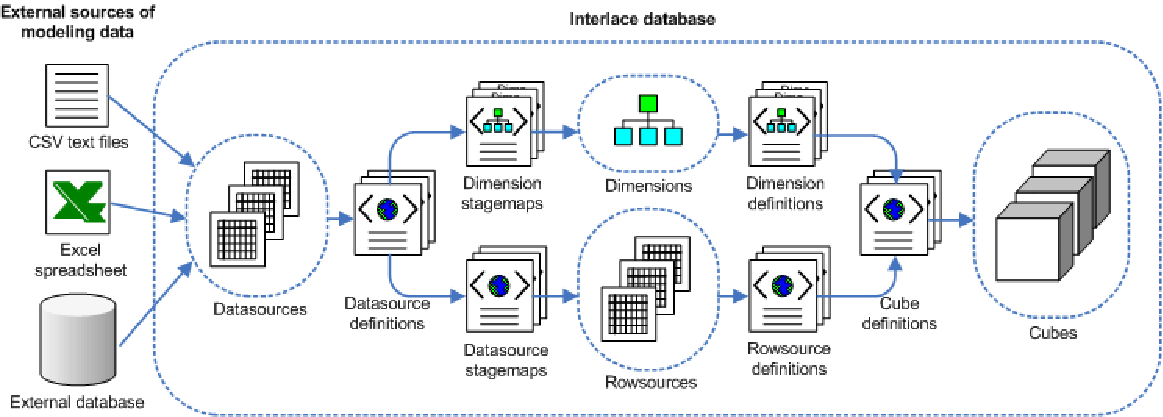
\includegraphics[width=\linewidth]{figures/data-mapping.pdf}
	\caption{Mapping and Modeling Data from Diverse Sources}
    \floatfoot{Source: Oracle User's Guide}
	\label{fig:mapping}
\end{figure}

Figure \ref{fig:mapping} illustrates the relationship and the flow of data among various modeling elements:
%
as we can see, users can model data either creating a model using the data designer integrated in the system or importing a model using XML meatadata definition files.
%
The data coming from different sources is loaded into data-sources, which are relational tables in the integrated planning database where copies of external modeling data are stored. 
%
According to the data-source definitions, the columns to use are set, while stage maps map data-sources to row sources or dimensions in the planning database. 
%
One data-source can be mapped to more than one row source.
%
When data-sources are mapped to dimensions, the system maps the names from the tabular data-source to the elements of the dimension’s hierarchical structure. 
%
In addition to mapping columns to dimension members at all levels, the system maps the attributes of the dimension members and specifies the relationship (for example, parent-child).
%
The mapping among cubes allows data values in one cube to flow to data values in another cube. 
%
Since the cubes have different structures, the mapping defines how the data should flow; the mapping is like a table join in a relational database: it defines the common dimensions and how to map or join them.

To identify how source dimensionality translates to target dimensionality, member mappings based on source values are used. 
%
Member mappings are referenced during the data load, enabling the Data Management to determine how to dimensionalize the data that is loaded to the target application. 
%
They define relationships between source members and target dimension members within a single dimension. 
%
This is done by creating a member mapping for each target dimension which, based on the business logic, can have different levels of granularity:

\begin{enumerate}
    \item Explicit: the source value is matched exactly and replaced with the target value. For example, source value ``ABC'' is replaced with target value ``123''.
    \item Between: the range of source values is replaced with a single target value. For example, a range from ``001'' to ``010'' is replaced as one value: ``999''. 
    \item In: it enables a list of non-sequential source values to be mapped to one target value. For example, you could have source accounts 1503, 1510, and 1515 map to the target account 15000010.
    \item Multi-Dimension: it enables users to define member mapping based on multiple source column values. For example, if the source value combination is Entity-001,002 Department-ABC, XYZ Account-1222, 1333, then the target value assigned for Account Dimension is 1200.
    \item Like: the string in the source value is matched and replaced with the target value.  For example, the source value ``Department'' is replaced with the target value ``Cost CenterA''.
\end{enumerate}

When processing the source values for transformations, multiple mappings may apply to a specific source value. 
%
The order of precedence is Explicit, Between, In, Multi-Dimension, and Like. 

Once data have been mapped into the correct dimensions and members, the next step is to transform them to match the requirements of FCCS. 
%
Data transformation is a critical aspect of data integration and management as it enables organizations to convert data from various source systems into a consistent format that can be used for financial consolidation and reporting.
%
This process involves applying various rules and calculations to ensure that data is accurate, complete and consistent.
%
More in details, some specific data transformation techniques used in FCCS include:

\begin{enumerate}
    \item Data Validation: Checking data for errors, inconsistencies, and missing values, and correcting or flagging issues as necessary.
    \item Data Aggregation:  Combining data at various levels of granularity to produce summary values for reporting and analysis.
    \item Data Translation: Converting data from one language or currency to another to facilitate consolidation and reporting.
    \item Intercompany Elimination: Adjusting data to eliminate transactions between related entities or companies, in order to produce accurate consolidated financial statements.
\end{enumerate}

FCCS provides a range of tools and features to support data transformation, including pre-built mapping templates, data validation rules, and built-in calculations and consolidation methods. 
%
At the same time, this application provides a range of features to help users manage data governance.
%
This aspect is particularly important for a Holding Group as it helps ensuring that data is managed and protected consistently across all entities, while guaranteeing that data usage is compliant with regulations and best practices.
%
Effective data governance ensures that data is managed and protected, while being compliant with regulations such as GDPR, the Italian Data Protection Law, and CCPA \footnote{The GDPR (General Data Protection Regulation) applies to any company that processes the personal data of individuals located in the European Union, regardless of where the company is located. The Holding Group must also comply with the Italian Data Protection Law, which regulates the processing of personal data in Italy, as well as other data protection regulations in the countries where its brands are located, including U.S with the CCPA (California Consumer Privacy Act).}, reducing the risk of penalties, fines, or legal actions.
%
At the same time, it ensures that sensitive data is protected from unauthorized access,  reducing the risk of data breaches and consequential reputational damage.
%
On a more technical level, data governance ensures that data is shared in a controlled and secure manner, while ensuring that data is managed and used consistently across all entities, improving standardization and efficiency.

The process of data load runs continuously to keep the EPM system up-to-date with respect to the financial situation of the Group in real-time.
%
It is therefore important to update the process systematically to meet changes in business operations and allow the system to run smoothly, providing an accurate representation of reality.
%
Oracle FCCS serves as a powerful tool within the EPM framework as it empowers organizations to streamline financial consolidation, close processes, and reporting. 

The process of consolidating financial data from multiple entities, business units and subsidiaries is automated, ensuring accurate and consistent consolidation by applying predefined rules, intercompany eliminations, currency translations, and other necessary adjustments.
%
At the same time, FCCS facilitates the entire close management process\footnote{The close management process refers to a series of activities undertaken by businesses to finalize their financial records for a specific period, typically at month-end, quarter-end, or year-end. It involves tasks such as reconciliations, adjusting entries, financial reporting, review and approval, and documentation.} by providing a centralized system to track, manage, and review the progress of close tasks. 
%
It allows organizations to define close calendars, assign responsibilities, and monitor the completion of close activities.
%
The integration capabilities of FCCS enable a smooth flow of data to other Oracle EPM solutions, such as Oracle Planning for planning, reporting and forecasting purposes - as shown in figure \ref{fig:planning-fccs}.
%
By seamlessly loading data from FCCS to the planning system, the Group can leverage the consolidated financial data for budgeting, forecasting, and scenario planning. 
%
This native integration ensures a cohesive and holistic approach to financial management, facilitating data-driven decision-making across the organizations.
%
Data from FCCS are copied periodically into Planning with specific rules set to keep data aligned between the two environments.
%
The import rule is automatic but it can also be launched at Group level. 

\begin{figure}[htbp]
	\centering
	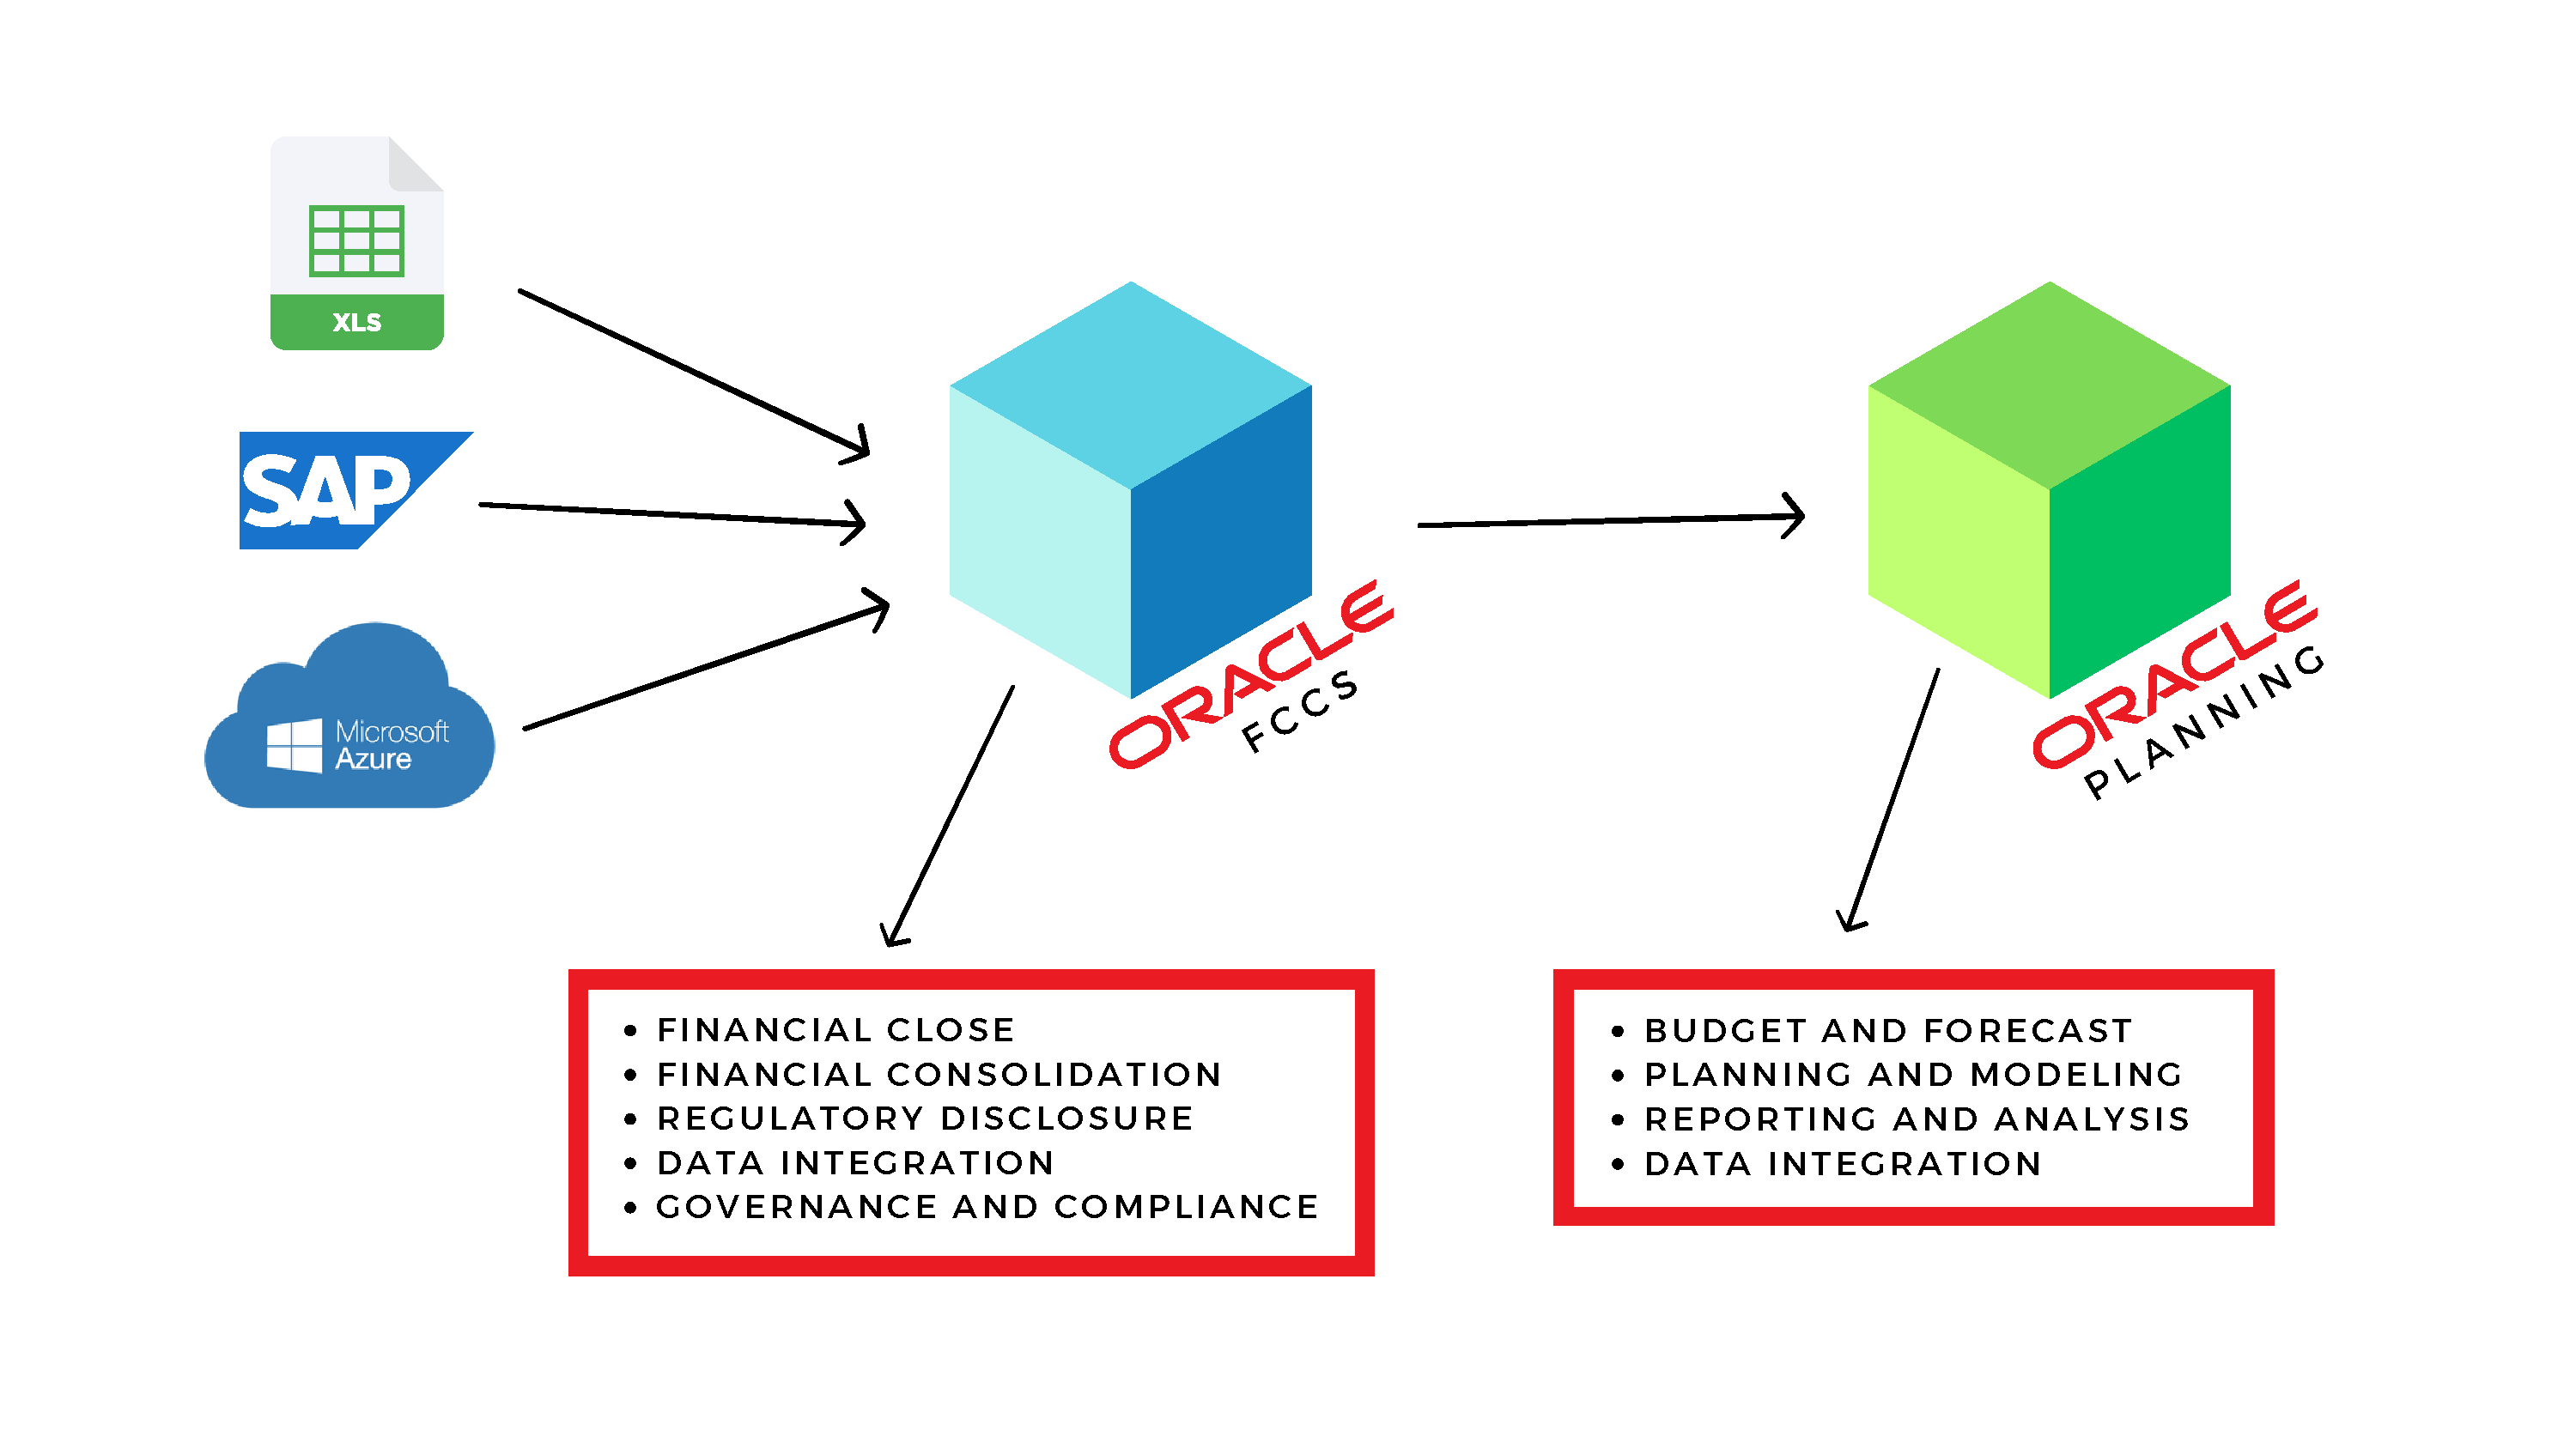
\includegraphics[width=\linewidth]{figures/planning-fccs.pdf}
	\caption{Integration between FCCS and Oracle Planning}
	\label{fig:planning-fccs}
\end{figure}

The integration between Oracle FCCS and Oracle Planning allows organizations to seamlessly transfer financial data from the consolidated financial system to the planning system. 
%
This automated data flow eliminates the need for manual data entry and reduces the risk of errors that can occur during manual data transfer.
%
By leveraging the data from Oracle FCCS, organizations can align their planning and budgeting processes with the actual financial results, as the system incorporates the most up-to-date and accurate financial information from the consolidation process.
%
The automatic data loading from FCCS to Oracle Planning ensures data integrity and consistency throughout the planning and budgeting cycle; any changes or updates made in the consolidated financial system are automatically reflected in the planning system, enabling users to work with real-time data for their budgeting and forecasting activities.
%
Furthermore, the automation of data loading from to Oracle Planning enhances the efficiency of the planning and budgeting process by reducing the time and effort required for data reconciliation and ensuring that the planning system is always synchronized with the latest financial information. 

Oracle Planning offers a robust set of functionalities that empower businesses to streamline their financial processes and make informed decisions. 
%
With activities like planning and modeling, budgeting and forecasting together with reporting and analysis, Oracle Planning provides a comprehensive suite of tools and features to support organizations in their journey towards optimized financial performance. 
%
 Let's explore the key functionalities of Oracle Planning in detail.

\paragraph{Planning and Modeling:} 

Planning and modeling refers to the process of creating strategic plans, setting goals, and developing models that simulate various business scenarios.
%
By modeling different scenarios, organizations can assess the potential impact of changes and make informed decisions based on those insights.
%
Oracle Planning allows users to create multiple planning scenarios to assess the impact of different business variables on financial outcomes, enabling organizations to evaluate various what-if scenarios and make informed decisions based on different assumptions.
%
Users can model and forecast financial results based on key business drivers such as sales volume, pricing or production capacity.
%
This approach helps organizations understand the relationships between drivers and financial outcomes.
%
Oracle Planning also includes specialized features for workforce planning and modeling which enable organizations to forecast and manage their human resources-related expenses, such as salaries, benefits, and workforce allocation, ensuring alignment between workforce planning and overall financial planning.

\paragraph{Budgeting and Forecasting:}

Budgeting and forecasting involve the creation of financial plans and projections for a specific period.
%
Budgeting focuses on allocating financial resources to different areas of the organization, while forecasting predicts future financial performance based on historical data and anticipated changes. 
%
Oracle Planning provides a user-friendly interface for creating and managing budgets: users can input, review, and adjust budget data, leveraging predefined templates and workflows to streamline the budgeting process. 
%
At the same time, organizations can perform rolling forecasts using Oracle Planning, allowing them to update and revise their forecasts periodically based on actual performance and changing business conditions. 
%
This helps to keep forecasts accurate and relevant throughout the planning period.

\paragraph{Reporting and Analysis:}

Reporting and analysis encompass the generation of financial statements, performance reports, and key performance indicators (KPIs) to assess the financial health and performance of an organization. 
%
Reporting and analysis facilitate data-driven decision-making, provide visibility into financial performance, and support effective communication with stakeholders.
%
Oracle Planning enables the generation of financial statements, including balance sheets, income statements, and cash flow statements: users can create customized reports that provide insights into financial performance, variances, and key metrics. 
%
The solution supports various reporting formats, including tabular reports, graphical dashboards, and interactive visualizations.
%
The system also empowers users to perform ad-hoc analysis by providing intuitive tools and interfaces. 
%
Users can explore data, drill down into details, create personalized views, and conduct multidimensional analysis to uncover trends, patterns, and outliers.
%
With Oracle Planning, organizations can analyze and compare actual performance against budgeted or forecasted figures in order to identify areas of variance and take corrective actions as necessary.
%
Finally, Oracle Planning offers interactive dashboards with real-time data visualizations and KPI monitoring that users can use to create personalized dashboards to track performance, monitor progress, and gain insights into key business metrics.

\section{Data transformations and calculations}

In Oracle Cloud EPM, data transformation and calculation are fundamental aspects that enable organizations to derive meaningful insights and make informed decisions. 
%
Within the EPM environment, these capabilities are achieved through the utilization of business rules.
%
This section delves into the world of data transformation and calculation in Oracle Cloud EPM, focusing on how business rules drive these processes.
%
Data transformation and calculation in Oracle Cloud EPM play a key role in aggregating, consolidating, and manipulating data across the multidimensional cubes of the EPM application.
%
Business rules serve as the mechanism to define and automate complex calculations, allowing organizations to streamline their financial modeling, scenario planning, and other analytical operations.
%
Within this section, we explore the specific programming language used for creating business rules, known as Calculation Manager Script. 
%
This proprietary language provides a robust set of functions, operators, and syntax elements tailored to the EPM environment, empowering users to construct intricate calculations with precision and flexibility.
%
Additionally, this section elucidates the mechanics of how business rules operate across the multidimensional cubes. 
%
It explores the sequence and flow of calculations, the retrieval of data from source locations, and the storage of results in target locations, ensuring consistency and accuracy throughout the EPM application.

In Oracle Cloud EPM, data transformation and calculation capabilities are achieved through the use of business rules. 
%
Business rules provide a powerful mechanism for defining and automating complex calculations, data transformations, and validation logic within the multidimensional cubes of the EPM application.
%
The main elements of a business rule in Oracle Cloud EPM include:

\begin{enumerate}
    \item Rule Components: Business rules consist of various components, such as members, formulas, conditions, and data mappings. Members define the dimensions and hierarchy elements on which calculations are performed. Formulas define the mathematical or logical operations to be executed. Conditions allow for the application of calculations based on specific criteria. Data mappings define the source and target locations for data transformations.
    \item Functions and Operators: Calculation Manager Script provides a wide range of built-in functions and operators that enable complex calculations. These include mathematical functions (e.g., SUM, AVG, MAX), string functions, date functions, logical operators (e.g., IF-THEN-ELSE), and more. These functions and operators allow for the manipulation and transformation of data within the multidimensional cubes.
    \item Calculation Logic: Business rules define the sequence and flow of calculations. They specify how data is aggregated, allocated, consolidated, or transformed across dimensions within the OLAP cubes. Calculation logic can involve multiple steps, nested formulas, and conditional statements to perform calculations at different levels of aggregation.
\end{enumerate}

Business rules operate across the multidimensional cubes of the EPM application by applying calculations to specific intersections of dimensions. 
%
The rules are executed during the data consolidation and aggregation processes, allowing for real-time calculations and updates to the cube data.
%
When a business rule is triggered, it retrieves data from the specified source locations, performs the defined calculations using the specified logic and formulas, and then stores the results in the target locations within the multidimensional cube. 
%
This process ensures consistent and accurate calculations across the entire EPM application.

%----------------------------------------------------------------------------------------
\chapter{\conclusionsname}
\label{chap:conclusions}
%----------------------------------------------------------------------------------------

\section{Summary of the project}

\section{Discussion and concluding thoughts}


%----------------------------------------------------------------------------------------
% BIBLIOGRAPHY
%----------------------------------------------------------------------------------------

\nocite{*} % uncomment this to show all the reference in the .bib file
\bibliographystyle{plain}
\bibliography{bibliography}


\end{document}